%\documentclass[aspectratio=169]{beamer}
\documentclass[aspectratio=169]{beamer} 
% \documentclass{beamer} 
%\documentclass[aspectratio=169,handout]{beamer} 
\setbeameroption{show notes on second screen=bottom}

\usepackage{bigints}

\usepackage{tikz}
\usetikzlibrary{shadows,fadings,calc,patterns,positioning}
\usetikzlibrary{arrows.meta}
\tikzset{>={Latex[width=3mm,length=3mm]}}

\usepackage{pgfplots}
\pgfplotsset{compat=1.18}
\usepgfplotslibrary{groupplots}

\usepackage{microtype}
\usepackage[style=authoryear-comp,backend=biber]{biblatex}
\addbibresource{biblio.bib}

\usepackage{caption}

\usepackage{graphicx}   % graphics
\graphicspath{{./figures/}}
\usepackage{svg}

\usepackage{booktabs}

\usepackage{tikz}
\usetikzlibrary{shadows,fadings,calc}

\usepackage{minted}

\tikzfading[name=fade up, bottom color=transparent!0, top color=transparent!100]

\usepackage{appendixnumberbeamer}

\definecolor{wong_blue}{RGB}{0, 114, 178} % #0072B2
\definecolor{wong_orange}{RGB}{230, 159, 0} % #E69F00
\definecolor{wong_green}{RGB}{0, 158, 115} % #009E73
\definecolor{wong_purple}{RGB}{204, 121, 167} % #CC79A7
\definecolor{wong_skyblue}{RGB}{86, 180, 233} % #56B4E9
\definecolor{wong_vermillion}{RGB}{213, 94, 0} % #D55E00
\definecolor{wong_yellow}{RGB}{240, 228, 66} % #F0E442

\hypersetup{colorlinks,linkcolor=,urlcolor=wong_blue,citecolor=wong_purple}

\DeclareMathOperator{\erf}{erf}

\setkeys{Gin}{width=.75\textwidth, height=.75\textheight, keepaspectratio}

\newcommand\blfootnote[1]{%
  \begingroup
  \renewcommand\thefootnote{}\footnote{#1}%
  \addtocounter{footnote}{-1}%
  \endgroup
}

\usepackage{xspace}
\newcommand{\libsvm}{\texttt{libsvm}\xspace}
\newcommand{\x}{{\boldsymbol{x}}}
\newcommand{\y}{{\boldsymbol{y}}}
\newcommand{\z}{{\boldsymbol{z}}}

\usetheme{metropolis}

\pgfplotsset{cycle list={wong_blue,wong_orange,wong_green,wong_purple,wong_skyblue,wong_vermillion,wong_yellow}}

% \setbeamercolor{background canvas}{bg=white}
\setbeamertemplate{caption}[default]

\setbeamercolor{progress bar}{fg=wong_blue,bg=lightgray}

\title{I'll See You In the Limit:}
\subtitle{Understanding the Effects of Infinite Neural Network Kernels}
\date{October 19, 2023}
\author{Aleix Bon\'e}
\institute{
    \textbf{Degree:} Master's Degree in Data Science \\
    \textbf{Thesis supervisor:} Lluís Antonio Belanche-Muñoz (Department of Computer Science)
    \\[2em]
    \textbf{Facultat d’Informàtica de Barcelona (FIB)} \\
    \textbf{Universitat Politècnica de Catalunya (UPC) \textendash{} BarcelonaTech}
}

\titlegraphic{
	\tikz [remember picture,overlay]
	\node at
	([xshift=-3.25cm, yshift=+1.8cm]current page.south east)
	{
\includegraphics[width=0.4\textwidth]{logo-upc}};
}

\begin{document}
\maketitle

\centering

\section{Introduction}

\begin{frame}{Introduction \textendash{} \textcite{frenayParameterinsensitiveKernelExtreme2011}}
	\begin{center}
		\tikz\node [drop shadow]
		{\fcolorbox{black}{white}{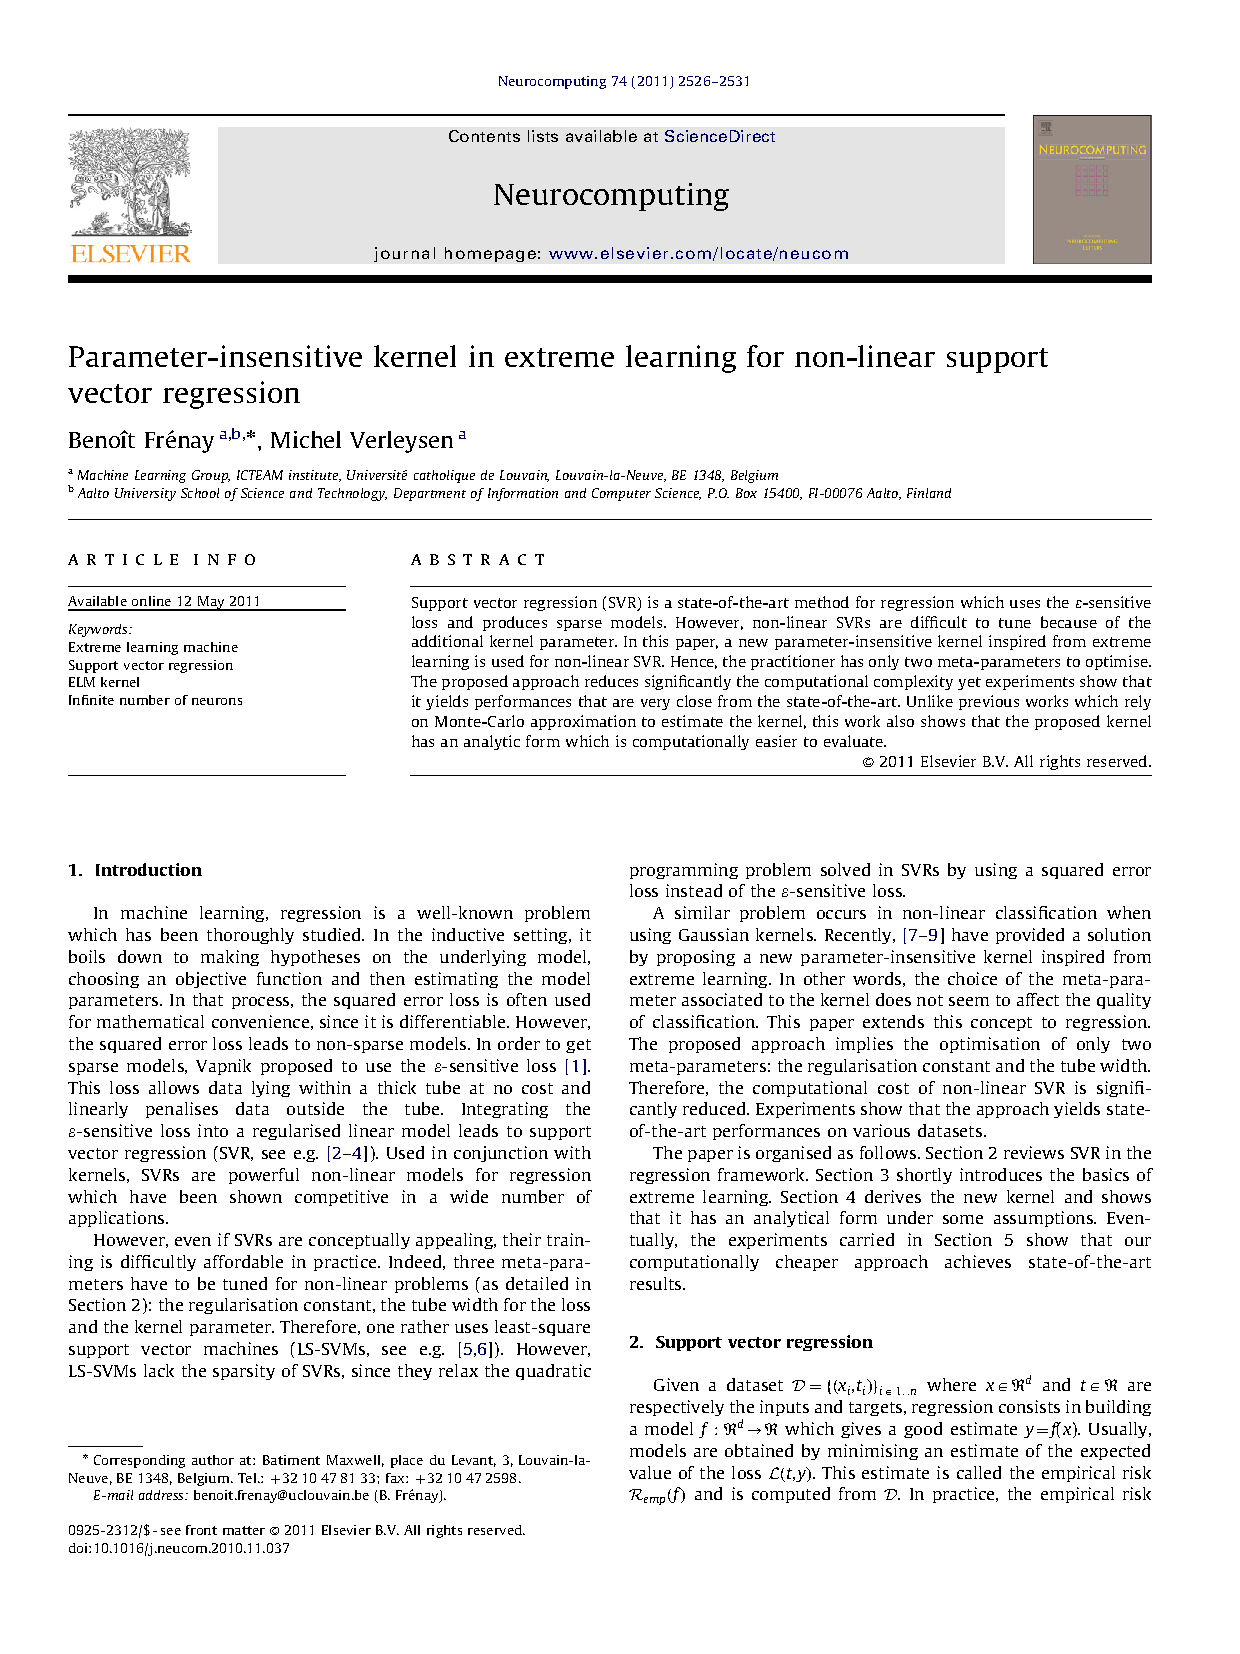
\includegraphics[width=0.8\textwidth,height=!]{frenay_paper}}};
	\end{center}
	\begin{tikzpicture}[overlay,remember picture]
		\coordinate (A) at ($(current page.south east) + (0, 0.5cm)$);
		\fill[color=normal text.bg, path fading=fade up] (current page.west) rectangle ($(A) - (0, 0.01cm)$);
		\fill[color=normal text.bg] (current page.south west) rectangle (A);
	\end{tikzpicture}
	\blfootnote{\fullcite{frenayParameterinsensitiveKernelExtreme2011}}
\end{frame}

\note[itemize]{
	\item \Textcite{frenayParameterinsensitiveKernelExtreme2011} presented a
	``parameter-insensitive'' kernel inspired from extreme learning machines.
	\item The meta-parameter associated with the kernel, once it reaches a certain threshold,
	further increasing its value
	does \emph{not affect} the performance of the results.
	\item They demonstrate effectiveness of the kernel in a Support Vector Regression task.
	\item Not significantly different from \emph{state-of-the-art} using Gaussian kernels.
	\item Seeing these results, we wonder if this property is also present in other
	infinite neural network kernels to some extent.
}

\begin{frame}{Introduction \textendash{} Goals}
	\begin{itemize}
		\item Study the effects of infinite neural network kernels
		\item Focusing on the dependence (or lack of) of performance on the kernel hyperparameters
	\end{itemize}
\end{frame}

\note{
	The aim of this project is to study the effects of these infinite neural network
	kernels in support vector machines; understanding their behaviour in practical
	learning problems, with a special focus on the dependence (or lack of) of
	performance on the kernel
	hyperparameters.

	Having a parameter-insensitive kernel has the potential to cut down on the time
	spent on hyperparameter tuning, which is one of the most time-consuming tasks in
	machine learning.
}

\begin{frame}{Introduction \textendash{} Methodology}
	\begin{enumerate}
		\item Research known infinite neural network kernels in the literature.
		\item Implement the kernels in \libsvm.
		\item Collect suitable datasets.
		\item Design and run experiments.
		\item Analyze the results.
	\end{enumerate}
\end{frame}

\section{Theoretical Background}

\begin{frame}{Theoretical Background \textendash{} Kernel Function}
	A kernel function is a function $k$ that, given two vectors $\boldsymbol x$ and $\boldsymbol y$ in a
	vector space $\mathcal{X}$, returns the inner product of their images in a
	feature space $\mathcal{H}$:
	\begin{equation*}
		k(\boldsymbol x,\, \boldsymbol y) = \left\langle \phi(\boldsymbol x),\, \phi(\boldsymbol y) \right\rangle_{\mathcal{H}}
	\end{equation*}
	where $\phi$ is a mapping from $\mathcal{X}$ to $\mathcal{H}$.
\end{frame}
\note[itemize]{
	\item Such a mapping $\phi$ is called a \emph{feature map}.
	\item $\mathcal{H}$ is an inner product space, and is called the
	\emph{reproducing kernel Hilbert space} (RKHS).
	\item These functions can be used to define a similarity measure.
	\item They can be used in machine learning algorithms such as support vector machines,
	allowing them to operate in a high-dimensional, implicit feature space without
	ever computing the coordinates of the data in that space.
	\item We call learning algorithms that accept kernels \emph{kernel methods}.
}
\begin{frame}{Theoretical Background \textendash{} Single Layer Feed-Forward Neural Network}
	\begin{figure}[htpb]
		% Single layer feedforward network
		\resizebox{.8\textwidth}{!}{
			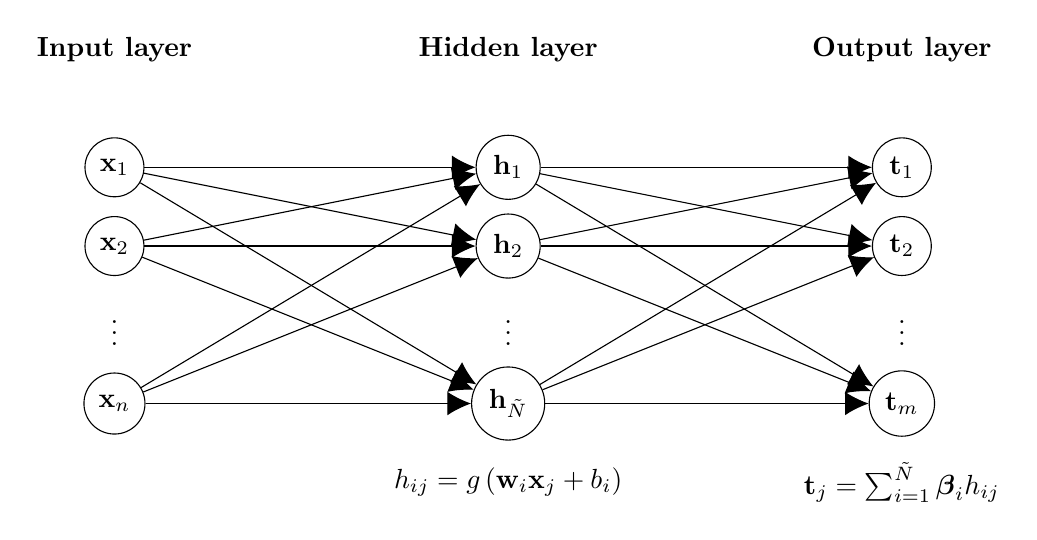
\begin{tikzpicture}
				% input layer
				\node[draw, circle] (x1) at (0, 0) {$\textbf x_1$};
				\node[draw, circle] (x2) at (0, -1) {$\textbf x_2$};
				\node (x3) at (0, -2) {$\vdots$};
				\node[draw, circle] (x4) at (0, -3) {$\textbf x_n$};

				% hidden layer
				\node[draw, circle] (h1) at (5, 0) {$\textbf h_1$};
				\node[draw, circle] (h2) at (5, -1) {$\textbf h_2$};
				\node (h3) at (5, -2) {$\vdots$};
				\node[draw, circle] (h4) at (5, -3) {$\textbf h_{\tilde{N}}$};

				% output layer
				\node[draw, circle] (y1) at (10, 0) {$\textbf t_1$};
				\node[draw, circle] (y2) at (10, -1) {$\textbf t_2$};
				\node (y3) at (10, -2) {$\vdots$};
				\node[draw, circle] (y4) at (10, -3) {$\textbf t_m$};

				\node (xtitle) at (0, 1.5) {\textbf{Input layer}};
				\node (htitle) at (5, 1.5) {\textbf{Hidden layer}};
				\node (ytitle) at (10, 1.5) {\textbf{Output layer}};

				\node (hformula) at (5, -4) {$h_{ij} = g \left( \textbf{w}_i \textbf{x}_j + b_i \right)$};
				\node (yformula) at (10, -4) {$\textbf{t}_{j} = \sum_{i=1}^{\tilde{N}} \boldsymbol\beta_{i} h_{ij}$};

				% connections
				\foreach \i in {1,2,4}
				\foreach \j in {1,2,4} {
						\draw[->] (x\i) -- (h\j);
						\draw[->] (h\i) -- (y\j);
					}
			\end{tikzpicture}
		}
		\caption{Single layer feedforward network}%
	\end{figure}
\end{frame}

\note[itemize]{
	\item $g$ is the activation function, which is applied element-wise to the
	weighted sum of the inputs to the neuron.
	\item $\boldsymbol w_i$ is the weight vector of the $i$-th neuron.
	\item $b_i$ is the bias of the $i$-th neuron.
	\item $\boldsymbol\beta_i$ is the weight vector of the $i$-th output neuron.
}

\begin{frame}{Theoretical Background \textendash{} Activation Function}
	\begin{figure}[H]
		\begin{tikzpicture}
			\begin{groupplot}[group style={
							group size=3 by 1,
							xlabels at=edge bottom,
							ylabels at=edge left,
							vertical sep=4em,
						},
					width = .3\textwidth,
					ymin=-0.1, ymax=1.1,
					every axis plot/.append style={mark=none, line width=2pt},
					enlarge x limits=false,
					samples=25,
					domain=-10:10,
					xmin=-10, xmax=10,
					grid=both,
					grid style={dotted, draw=gray!40, line width=1.0pt}
				]
				\nextgroupplot[title={\bfseries ReLU},xmin=-2,xmax=2]
				\addplot[color=wong_blue] gnuplot[id=relu]{x > 0 ? x : 0};

				\nextgroupplot[title={\bfseries Sigmoid }]
				\addplot[color=wong_orange,smooth] gnuplot[id=sigmoid]{exp(x)/(1 + exp(x))};

				\nextgroupplot[title={\bfseries tanh },ymin=-1,xmin=-5,xmax=5]
				\addplot[color=wong_green,smooth] gnuplot[id=tanh]{tanh(x)};
			\end{groupplot}
		\end{tikzpicture}
		\caption{Activation functions often used in neural networks}
		\label{fig:common_activation_functions}
	\end{figure}
\end{frame}

\begin{frame}{Theoretical Background \textendash{} Extreme Learning Machines (I)}
	Introduced by \textcite{huangExtremeLearningMachine2006}, Extreme Learning
	Machines (ELMs) are an alternative approach to training Single Layer Feed-forward
	Neural Networks (SLFNs):
	\begin{itemize}
		\item Randomly initialize the weights and biases of the hidden layer ($\boldsymbol w_i$ and $b_i$).
		\item Compute the output weights ($\boldsymbol\beta_i$) as: $\boldsymbol\beta = \boldsymbol H^\dagger \boldsymbol T$.
	\end{itemize}
\end{frame}
\note[itemize]{
	\item $\boldsymbol H$ is the hidden layer output matrix, and $\boldsymbol T$ is the target matrix.
	\item $\boldsymbol H^\dagger$ is the Moore-Penrose pseudoinverse of $\boldsymbol H$.
	\item Works with infinitely differentiable activation functions.
}

\begin{frame}{Theoretical Background \textendash{} Extreme Learning Machines (II)}
	\begin{columns}
		\begin{column}{0.4\textwidth}
			\textbf{Pros:}
			\begin{itemize}
				\item Fast training.
				\item Good generalization.
				\item No local minima.
			\end{itemize}
		\end{column}
		\begin{column}{0.4\textwidth}
			\textbf{Cons:}
			\begin{itemize}
				\item No control over the hidden layer.
				\item Underfitting and Overfitting issues.
				\item Dependent on the number of hidden neurons.
			\end{itemize}
		\end{column}
	\end{columns}
\end{frame}
\note{
	Some form of cross-validation is needed to determine the number of hidden neurons.
}


\begin{frame}{Theoretical Background \textendash{} ELM (arcsin) kernel (I)}
	\textcite{frenayParameterinsensitiveKernelExtreme2011} consider a kernel
	in which its feature map $\phi$ is that of an ELM with $p$ hidden nodes and \emph{erf} activation function.
	\begin{columns}
		\begin{column}{0.4\textwidth}
			\begin{align*}
				k(\boldsymbol x,\, \boldsymbol y,\,p) & = \frac{1}{p} \left\langle \phi(\boldsymbol x),\, \phi(\boldsymbol y) \right\rangle_{\mathcal{H}} \\[1em]
				\erf(x)                               & = \frac{2}{\sqrt{\pi}} \int_{0}^{x} e^{-t^2} dt
			\end{align*}
		\end{column}
		\begin{column}{0.6\textwidth}
			\begin{figure}[H]
				\begin{tikzpicture}
					\begin{axis}[
							every axis plot/.append style={smooth, mark=none, line width=1.5pt, domain=-3:3, samples=50, no markers},
							enlarge x limits=false,
							legend pos=north west,
							height=4.5cm,
							width=0.9\textwidth,
							grid=both,
							grid style={dotted, draw=gray!40, line width=1.0pt}
						]
						\addplot+ gnuplot[id=erf]{erf(x)};
						\addlegendentry{$\erf(x)$};
						\addplot+[dashed] gnuplot[id=tanh]{tanh(x)};
						\addlegendentry{$\tanh(x)$};
					\end{axis}
				\end{tikzpicture}
				\caption{\emph{erf} and \emph{tanh} are very similar}
			\end{figure}
		\end{column}
	\end{columns}
\end{frame}

\begin{frame}{Theoretical Background \textendash{} ELM (arcsin) kernel (II)}
	At the limit of $p \to + \infty$, the kernel function is equivalent to the one
	proposed by \textcite{williamsComputingInfiniteNetworks1996} from the context of
	Bayesian Neural Networks (BNNs):
	\begin{equation}
		k(\boldsymbol x,\,\z \mid p \to + \infty)  = \frac{2}{\pi}
		\arcsin \frac{1 + \left\langle \boldsymbol x,\,\z \right\rangle}{\sqrt{
				\left(
				\frac{1}{2\sigma_w^2} + 1 + \left\langle \boldsymbol x,\,\boldsymbol x \right\rangle
				\right)
				\left(
				\frac{1}{2\sigma_w^2} + 1 + \left\langle \z,\,\z \right\rangle
				\right)
			}}
	\end{equation}
	where $\sigma_w^2$ is the variance of the weights \footnote{
		More precisely, $\sigma_w^2$ is the variance of Gaussian distribution with 0 mean from which the weights and biases of the
		hidden layer are drawn.
	}
\end{frame}
\note{
	Where $\sigma_w^2$ is the variance of Gaussian distribution with 0 mean from which the weights and biases of the
	hidden layer are drawn.
}

\begin{frame}{Theoretical Background \textendash{} Arccosine kernel (I)}
	\textcite{choLargemarginClassificationInfinite2010} generalize the work of
	\textcite{williamsComputingInfiniteNetworks1996} by considering alternative activation functions:
	\begin{align*}
		k_n(\boldsymbol x, \y) & = 2 \bigintss \frac{\exp\left(-\frac{\lVert \textbf w \rVert^2}{2}\right)}{(2\pi)^{d/2}}
		\Theta(\textbf w \cdot \boldsymbol x) \Theta(\textbf w \cdot \y) (\textbf w \cdot \boldsymbol x)^n (\textbf w \cdot \y)^n \,d\textbf w \\
		\intertext{where: }
		\Theta(z)              & = \frac{1}{2} \bigl(1 + \text{sign}(z)\bigr)                                                                  \\
		\intertext{and the activation function is: }
		g(z)                   & = \Theta(z)z^n
	\end{align*}
\end{frame}

\begin{frame}{Theoretical Background \textendash{} Arccosine kernel (II)}
	\begin{figure}[H]
		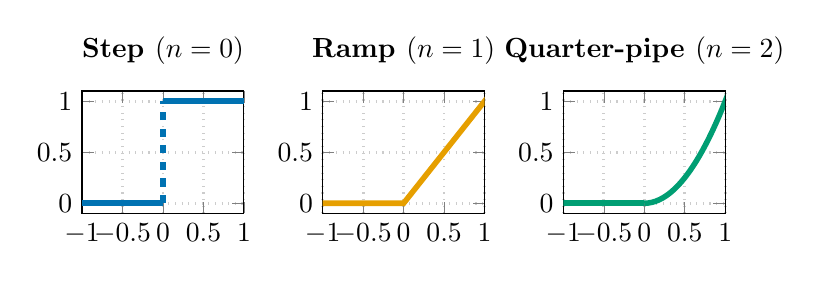
\begin{tikzpicture}
			\begin{groupplot}[group style={
							group size=3 by 1,
							xlabels at=edge bottom,
							ylabels at=edge left,
							vertical sep=4em,
						},
					width = .3\textwidth,
					ymin=-0.1, ymax=1.1,
					every axis plot/.append style={smooth, mark=none, line width=2pt},
					enlarge x limits=false,
					samples=25,
					domain=-1:1,
					xmin=-1, xmax=1,
					grid=both,
					grid style={dotted, draw=gray!40, line width=1.0pt}
				]
				\nextgroupplot[title={\bfseries Step $(n = 0)$}]
				\draw[line width=2pt, color=wong_blue] (axis cs:-1,0) -- (axis cs:0,0);
				\draw[line width=2pt, color=wong_blue, dashed] (axis cs:0,0) -- (axis cs:0,1);
				\draw[line width=2pt, color=wong_blue] (axis cs:0,1) -- (axis cs:1,1);

				\nextgroupplot[title={\bfseries Ramp $(n=1)$}]
				\draw[line width=2pt, color=wong_orange] (axis cs:-1,0) -- (axis cs:0,0) -- (axis cs:1.1,1.1);

				\nextgroupplot[title={\bfseries Quarter-pipe $(n=2)$}]
				\draw[line width=2pt, color=wong_green] (axis cs:-1,0) -- (axis cs:0,0);
				\addplot[domain=0:1.1, line width=2pt, color=wong_green] {x^2};
			\end{groupplot}
		\end{tikzpicture}
		\caption{Activation functions $\Theta(z)z^n$ for $n = 0,\,1,\,2$}
		\label{fig:activation_functions}
	\end{figure}
\end{frame}

\begin{frame}{Theoretical Background \textendash{} Arccosine kernel (III)}
	\begin{align}
		k_n(\boldsymbol x,\,\y) & = \frac{1}{\pi} \left\lVert \boldsymbol x \right\rVert^n \left\lVert \y \right\rVert^n J_n(\theta)                                                \\[1em]
		J_n(\theta)             & = (-1)^n \left( \sin \theta \right)^{(2n+1)}
		\left( \frac{1}{\sin \theta} \frac{\partial}{\partial \theta} \right)^2
		\left( \frac{\pi - \theta}{\sin \theta} \right)
		% \quad \text{for} \quad \forall n \in \left\{ 0,\,1,\,2,\,\dots \right\}                                                                                                     
		\\
		\theta                  & = \arccos \left( \frac{\left\langle \boldsymbol x,\,\y \right\rangle}{\left\lVert \boldsymbol x \right\rVert \left\lVert \y \right\rVert} \right)
	\end{align}
\end{frame}
\begin{frame}{Theoretical Background \textendash{} Arccosine kernel (IV)}
	For $n = 0,\,1,\,2$, the expression for $J_n(\theta)$ is:
	\begin{align}
		J_0(\theta) & = \pi - \theta                                                                     \\
		J_1(\theta) & = \sin\theta + \left(\pi - \theta\right)\cos\theta               \label{eq:cho_j1} \\
		J_2(\theta) & = 3\sin\theta\cos\theta + \left(\pi - \theta\right)\left(1 + 2\cos^2\theta\right)
	\end{align}
\end{frame}

\begin{frame}{Theoretical Background \textendash{} Covariance Arccosine kernel}
	The kernel from \textcite{choLargemarginClassificationInfinite2010} is derived
	from a Gaussian distribution with mean 0 and variance 1.
	\textcite{pandeyGoDeepWide2014} show how to obtain a variant of the kernel
	with a different covariance matrix $\Sigma$:
	\begin{equation}\label{eq:kernel_pandey}
		K_{\Sigma,\,n}(\boldsymbol x,\,\y) = K_{n}\left(\Sigma^{\frac{1}{2}}\boldsymbol x,\,\Sigma^{\frac{1}{2}}\y\right)
	\end{equation}
\end{frame}

\begin{frame}{Theoretical Background \textendash{} Kernel normalization}
	\begin{equation}
		K'(\boldsymbol x,\,\y) = \frac{K(\boldsymbol x,\,\y)}{\sqrt{K(\boldsymbol x,\,\boldsymbol x)K(\y,\,\y)}}
	\end{equation}
	\begin{block}{Arccosine}
		For the arccosine kernel, when normalizing the kernel, it reduces to:\footnote{This has the effect of eliminating the $\Sigma$ term in the covariance kernel.}
		\begin{equation}
			K'_n(\boldsymbol x,\,\y) = \frac{J_n(\theta)}{\pi}, \quad \forall n \in \left\{ 0,\,1,\,2 \right\}.
		\end{equation}
	\end{block}
\end{frame}

\section{Implementation}

\begin{frame}{Implementation \textendash{} \libsvm}
	\libsvm \parencite{CC01a} is a library for Support Vector Machines (SVMs) that
	is widely used in the machine learning community.
	\begin{columns}
		\begin{column}{0.6\textwidth}
			\begin{itemize}
				\item Open source under the BSD\textendash{}3 license.
				\item Written in \emph{C++}.
				\item Well documented.
				\item Widely used (Python, R, Julia, \dots)
				\item No external dependencies (only \texttt{glibc}).
			\end{itemize}
		\end{column}
		\begin{column}{0.37\textwidth}
			\begin{figure}[H]
				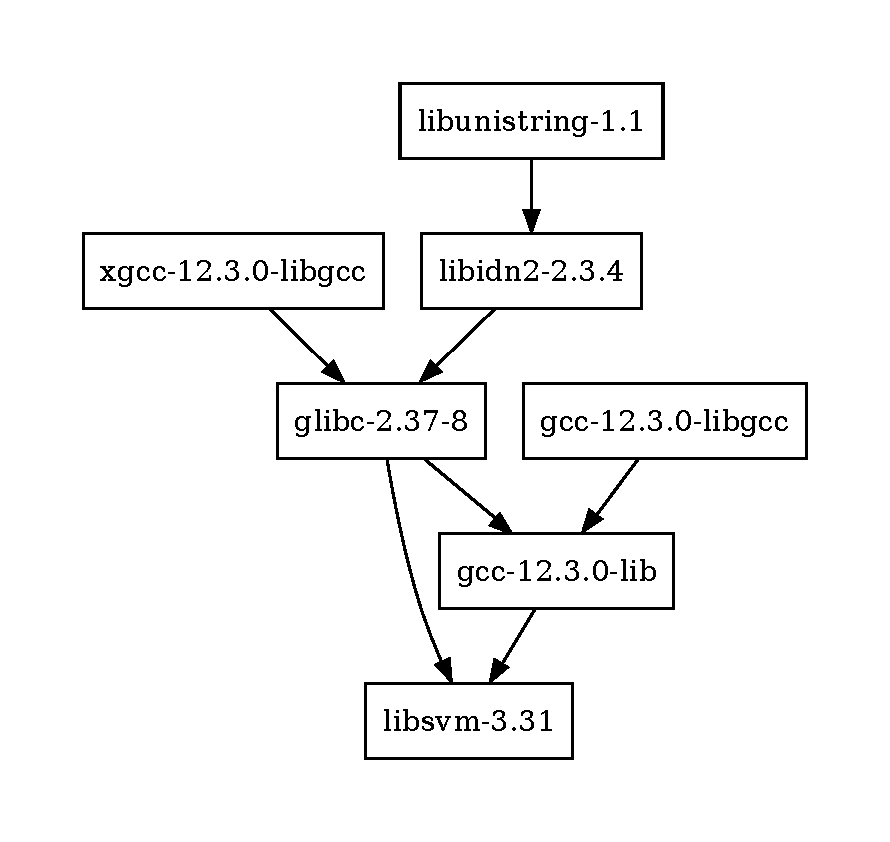
\includegraphics[width=.75\textwidth]{dependency_tree_libsvm}
				\caption{\libsvm dependencies.}
			\end{figure}
		\end{column}
	\end{columns}
\end{frame}

\begin{frame}{Implementation \textendash{} Julia}
	\begin{columns}
		\begin{column}{0.4\textwidth}
			\begin{figure}[H]
				
\includegraphics[width=.75\textwidth]{julia-logo-color}
			\end{figure}
			\url{https://julialang.org}
		\end{column}
		\begin{column}{0.4\textwidth}
			\begin{itemize}
				\item Fast
				\item Dynamic
				\item Reproducible
				\item Composable
				\item General
				\item Open source
			\end{itemize}
		\end{column}
	\end{columns}
\end{frame}
\note[itemize]{
	\item Julia is a high-level, high-performance, dynamic programming language.
	\item It is a general purpose language, and is designed to be easy to use for
	both numerical and general programming.
	\item The multiple dispatch paradigm allows extending the functionality of
	existing types without having to modify the original code.
	\item Joined the 1 PetaFLOP club in 2017 (Celeste.jl)
	\item Growing and active community.
}

\begin{frame}{Implementation \textendash{} Julia \textendash{} MLJ}
	% \begin{columns}
	% 	\begin{column}{0.6\textwidth}
	% 		\begin{itemize}
	%                \item \texttt{}
	%                \item \texttt{LIBSVM.jl}
	%                \item \texttt{MLJ.jl} (\texttt{MLJLIBSVMInterface.jl})
	% 		\end{itemize}
	% 	\end{column}
	% 	\begin{column}{0.4\textwidth}
	% 		\begin{figure}[H]
	% 			\includesvg[width=.75\textwidth]{MLJLogo2}
	% 		\end{figure}
	% 	\end{column}
	% \end{columns}
	\begin{figure}[H]
		\resizebox{0.9\textwidth}{!}{
			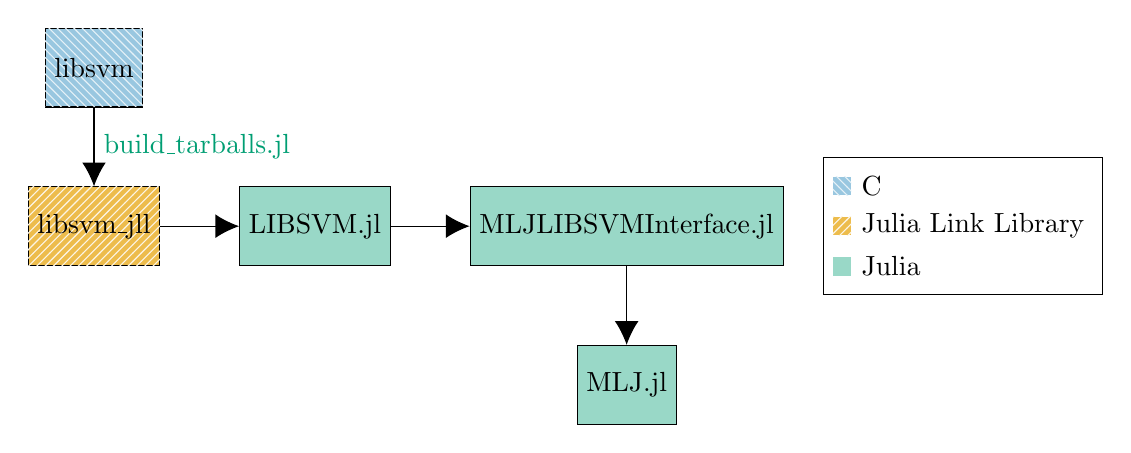
\begin{tikzpicture}[
					box/.style={draw, rectangle, minimum width=1cm, minimum height=1cm},
					C/.style={fill=wong_blue!40,postaction={pattern=north west lines,pattern color=wong_blue!10}},
					Julia/.style={fill=wong_green!40},
					JLL/.style={fill=wong_orange!70,postaction={pattern=north east lines,pattern color=wong_orange!10}},
				]
				\node[box,C] (libsvm) at (0,0) {libsvm};
				\node[box,JLL,below=of libsvm] (libsvm_jll) {libsvm\_jll};
				\node[box,Julia,right=of libsvm_jll] (LIBSVM) {LIBSVM.jl};
				\node[box,Julia,right=of LIBSVM] (MLJLIBSVMInterface) {MLJLIBSVMInterface.jl};
				\node[box,Julia,below=of MLJLIBSVMInterface] (MLJ) {MLJ.jl};

				\draw[->] (libsvm) -- (libsvm_jll) node[midway, anchor=west,color=wong_green] {build\_tarballs.jl};
				\draw[->] (libsvm_jll) -- (LIBSVM);
				\draw[->] (LIBSVM) -- (MLJLIBSVMInterface);
				\draw[->] (MLJLIBSVMInterface) -- (MLJ);

				% Color Legend
				\matrix [draw,right] at ($(current bounding box.east)+(0.5,0)$) {
					\node [C,label=right:C] {};                    \\
					\node [JLL,label=right:Julia Link Library] {}; \\
					\node [Julia,label=right:Julia] {};            \\
				};

			\end{tikzpicture}
		}
		% \caption{Dependency graph of Julia packages exposing the \libsvm library API.}
		% \label{fig:julia_libsvm_deps}
	\end{figure}
\end{frame}
\note[itemize]{
	\item \texttt{libsvm\_jll} is a Julia Link Library (JLL) package for \libsvm.
	\item \texttt{LIBSVM.jl} is a Julia wrapper for \libsvm.
	\item \texttt{MLJLIBSVMInterface.jl} is a Julia wrapper for \texttt{LIBSVM.jl} to make
	it compatible with \texttt{MLJ.jl}.
	\item \texttt{MLJ.jl} is a machine learning framework for Julia.
	\item Once we have our \libsvm fork integrated with MLJ, we can take advantage of
	the existing infrastructure to run experiments.
	\item \texttt{DrWatson.jl}, \texttt{Pluto.jl}, \texttt{Makie.jl} \dots
}

\section{Experiments}

\subsection{Setup}

\begin{frame}{Experiments \textendash{} $5\times{}2$ cross-validation}
	\begin{figure}[H]
		\resizebox{0.95\textwidth}{0.9\textheight}{
			%! TEX root = **/000-main.tex
% vim: spell spelllang=en:

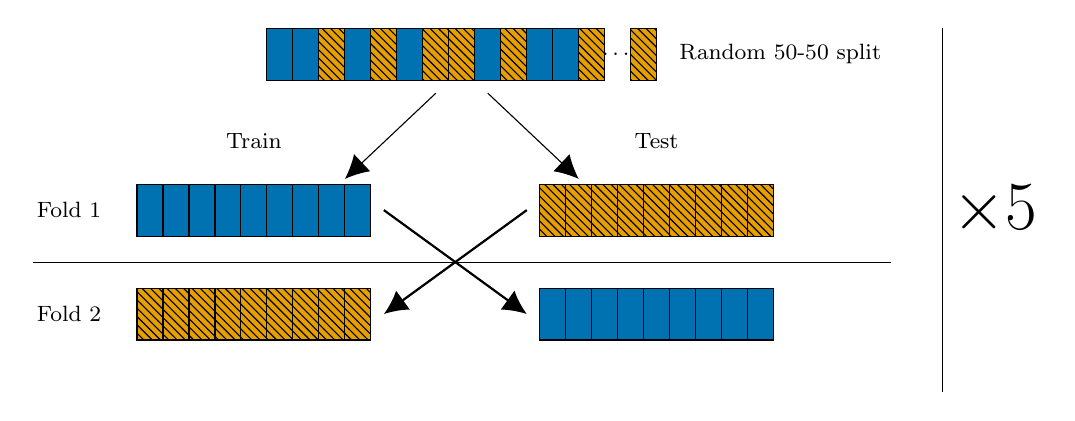
\begin{tikzpicture}[
		scale=0.66,
		every node/.style={font=\footnotesize},
	]
	% Draw main rectangle
	\def\nfolds{10}
	\pgfmathsetmacro{\trainfolds}{\nfolds-1}
	\pgfmathsetmacro{\splits}{\nfolds-2}
	\def\heightmult{0.5}

	\newcommand{\fold}[3]{%
		\draw[#2] #1 rectangle ($#1+(\heightmult*\trainfolds,1)$);
		\draw[#3] #1 rectangle ($#1+(\heightmult*\trainfolds,1)$);
		% fill with pattern

		% \draw ($#1+(\heightmult*\trainfolds/2,0)$) node[below,name=below-#5] {training set};
		% \draw ($#1+(\heightmult*\nfolds,0.5)$) node[right,name=right-#5] {#4 set};

		% Draw vertical dashed lines for fold divisions
		\foreach \x in {1,...,\splits}{
				\draw ($#1+(\heightmult*\x,0)$) -- ($#1+({\heightmult*\x},1)$);
			}
	}

	\def\coltest{wong_blue}
	\def\colvali{wong_orange}

	\filldraw[fill=\coltest] (-1,-1) rectangle (0,0);
	\filldraw[fill=\coltest] (-0.5,-1) rectangle (0,0);

	\filldraw[fill=\colvali] (0,-1) rectangle (0.5,0);
	\draw[pattern=north west lines] (0,-1) rectangle (0.5,0);

	\filldraw[fill=\coltest] (0.5,-1) rectangle (1,0);

	\filldraw[fill=\colvali] (1,-1) rectangle (1.5,0);
	\draw[pattern=north west lines] (1,-1) rectangle (1.5,0);

	\filldraw[fill=\coltest] (1.5,-1) rectangle (2,0);

	\filldraw[fill=\colvali] (2,-1) rectangle (2.5,0);
	\filldraw[fill=\colvali] (2.5,-1) rectangle (3,0);
	\draw[pattern=north west lines] (2,-1) rectangle (3,0);

	\filldraw[fill=\coltest] (3,-1) rectangle (3.5,0);

	\filldraw[fill=\colvali] (3.5,-1) rectangle (4,0);
	\draw[pattern=north west lines] (3.5,-1) rectangle (4,0);

	\filldraw[fill=\coltest] (4,-1) rectangle (4.5,0);
	\filldraw[fill=\coltest] (4.5,-1) rectangle (5,0);

	\draw[color=white,text=black] (5.5,-1) rectangle (6,0) node[midway] {\dots};
	\filldraw[fill=\colvali] (5,-1) rectangle (5.5,0);
	\draw[pattern=north west lines] (5,-1) rectangle (5.5,0);
	\filldraw[fill=\colvali] (6,-1) rectangle (6.5,0);
	\draw[pattern=north west lines] (6,-1) rectangle (6.5,0);

	\draw (6.75,-0.5) node[right] {Random 50-50 split};
	\draw[->] (2.25,-1.25) -- (0.5,-2.9);
	\draw[->] (3.25,-1.25) -- (5,-2.9);

	\fold{(-3.5,-4)}{fill=\coltest}{}
	\fold{(4.25,-4)}{fill=\colvali}{pattern=north west lines}

	\fold{(4.25,-6)}{fill=\coltest}{}
	\fold{(-3.5,-6)}{fill=\colvali}{pattern=north west lines}

	\draw (-1.25,-2.5) node[align=center, anchor=south] {Train};
	\draw (6.5,-2.5) node[align=center, anchor=south] {Test};

	\draw (-4,-3.5) node[align=center, anchor=east] {Fold 1};
	\draw (-4,-5.5) node[align=center, anchor=east] {Fold 2};

	\draw[thick,->] (1.25,-3.5) -- (4, -5.5);
	\draw[thick,->] (4,-3.5) -- (1.25, -5.5);

	\draw (-5.5, -4.5) -- (11, -4.5);

	\draw (12, 0) -- (12, -7) node[midway, right] {\Huge $\times 5$};

\end{tikzpicture}


		}
		% \caption{5\texttimes2 cross-validation method}%
	\end{figure}
\end{frame}

\begin{frame}{Experiments \textendash{} paired $t$\textendash{}test}
	By using $5\times{}2$ cross-validation, we can perform a paired $t$\textendash{}test
	as described by \textcite{dietterichApproximateStatisticalTests1998}.

	% TODO: CHECK THIS
	% WARN: this is confusing
	\begin{align}
		p^{(j)}   & = p_A^{(j)} - p_B^{(j)}                                                       \notag \\
		\bar{p}_i & = \frac{p_i^{(1)} + p_i^{(2)}}{2}                                             \notag \\
		s_i^2     & = \left(p_i^{(1)} - \bar{p}_i\right)^2 + \left(p_i^{(2)} - \bar{p}_i\right)^2 \notag \\[1em]
		t         & = \frac{p_1^{(1)}}{\sqrt{(1/5)\sum_{i=1}^5 s_i^2}}
	\end{align}

\end{frame}
\note[itemize]{
	\item This allows to compare the performance of two algorithms in a statistically
	significant way.
	\item The null hypothesis is that the difference in performance is 0.
	\item The alternative hypothesis is that the difference in performance is not 0.
	\item We can reject the null hypothesis if the $p$-value is less than a certain
	threshold $\alpha$, usually 0.05.
	\item $t$-student distribution with 5 degrees of freedom.
}

\begin{frame}{Experiments \textendash{} Normalization}
	\begin{description}
		\item[Data]: all features are normalized to have zero mean and unit variance, including the target variable.
		\item[Kernel]: the kernel is normalized as described earlier.
		\item[Measure]: We use \emph{Normalized Root Mean Square Error} as our measure.
		\item[Hyperparameter]: the hyperparameter $\sigma$ is normalized by the number of features.
	\end{description}
\end{frame}

\begin{frame}{Experiments \textendash{} Normalized Root Mean Square Error (nRMSE)}
	\begin{equation}
		nRMSE = \frac{1}{\sigma_{obs}}\sqrt{\frac{1}{n}\sum_{i=1}^n (y_i - \hat{y}_i)^2}
	\end{equation}
\end{frame}

\section{Results}

\begin{frame}{Results \textendash{} Reproducing \textcite{frenayParameterinsensitiveKernelExtreme2011}}
	\begin{columns}
		\begin{column}{0.47\textwidth}
			\centering \textbf{Original}
			\begin{figure}[H]
				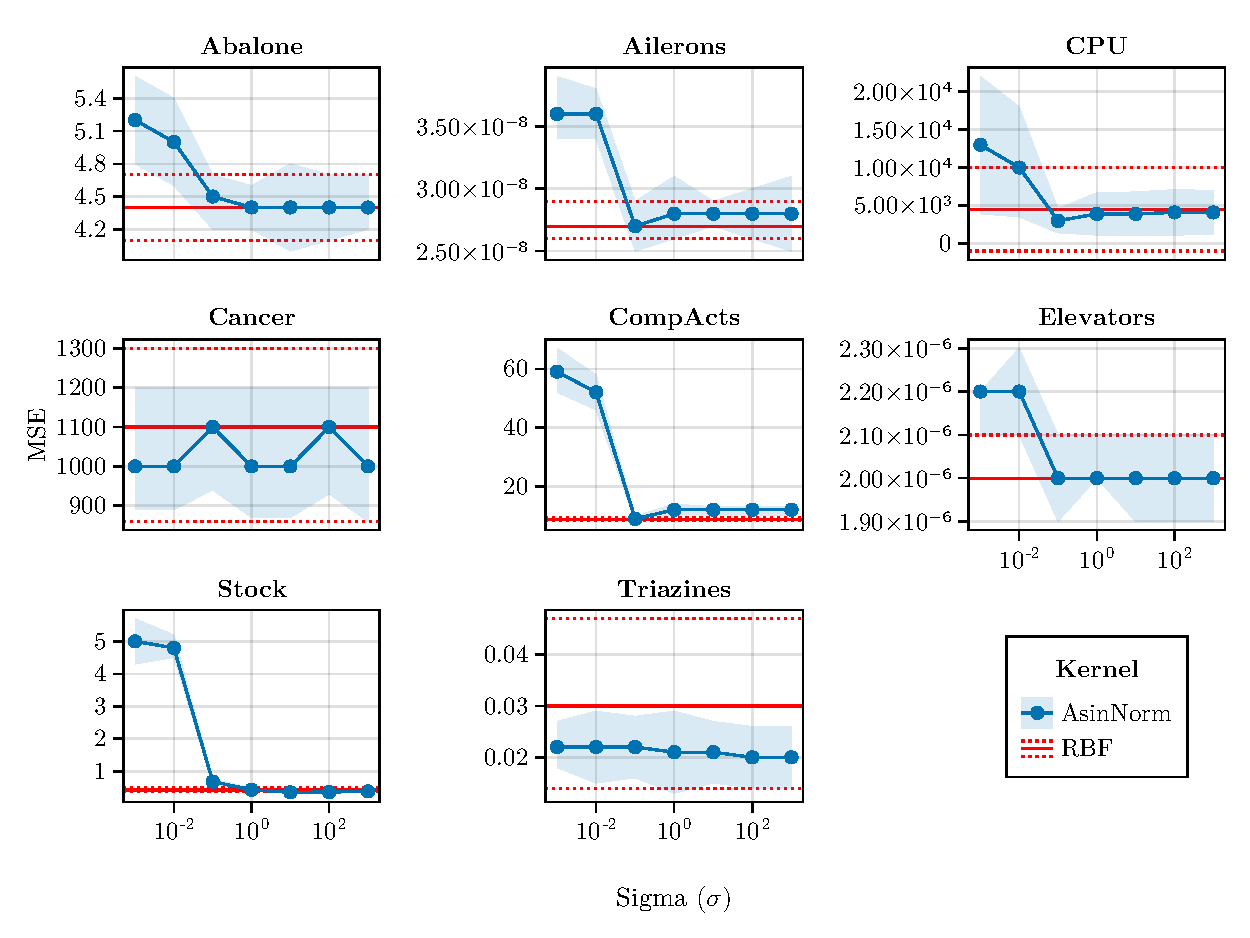
\includegraphics[width=\textwidth,height=0.95\textheight]{./figures/plots/MSE_frenay_original.pdf}
			\end{figure}
		\end{column}
		% \textrightarrow{}
		\begin{column}{0.47\textwidth}
			\centering \textbf{Reproduced}
			\begin{figure}[H]
				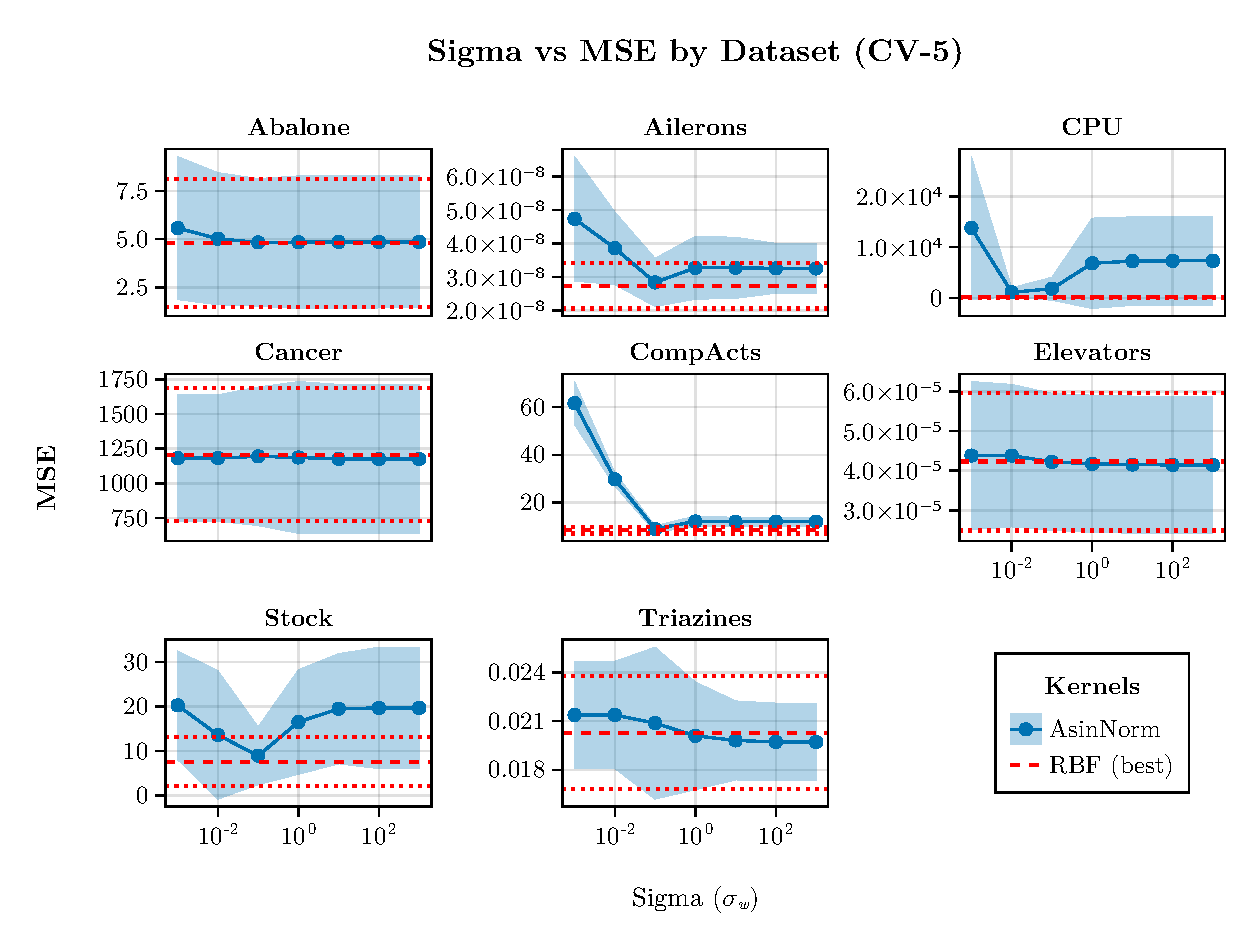
\includegraphics[width=\textwidth,height=0.95\textheight]{./figures/plots/MSE_frenay.pdf}
			\end{figure}
		\end{column}
	\end{columns}
\end{frame}

\begin{frame}{Results \textendash{} Normalized Arcsine kernel and RBF}
	\begin{figure}[H]
		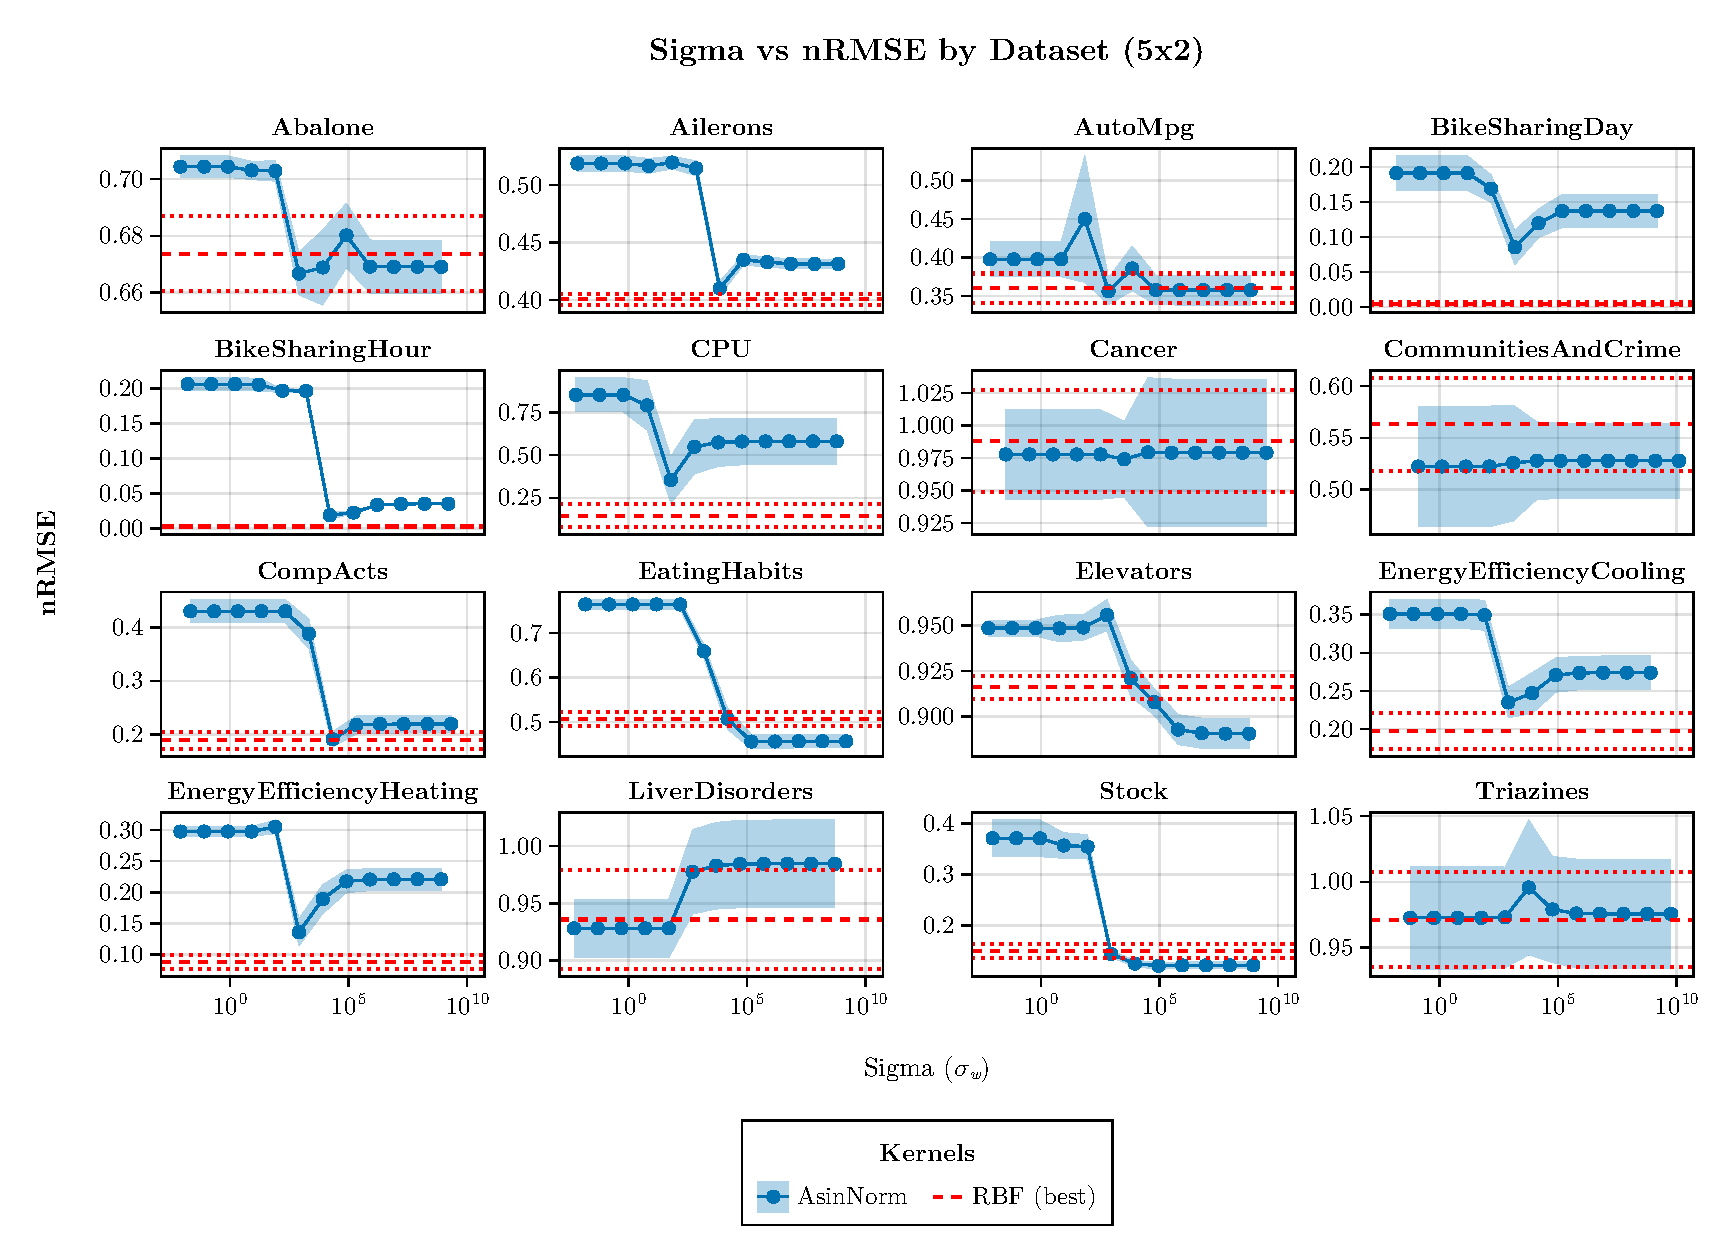
\includegraphics[width=\textwidth,height=0.95\textheight]{./figures/plots/nRMSE_nodelve_asinnorm_scaled_unlinked}
	\end{figure}
\end{frame}

\begin{frame}{Results \textendash{} Normalized Arcsine kernel and RBF (Delve)}
	\begin{figure}[H]
		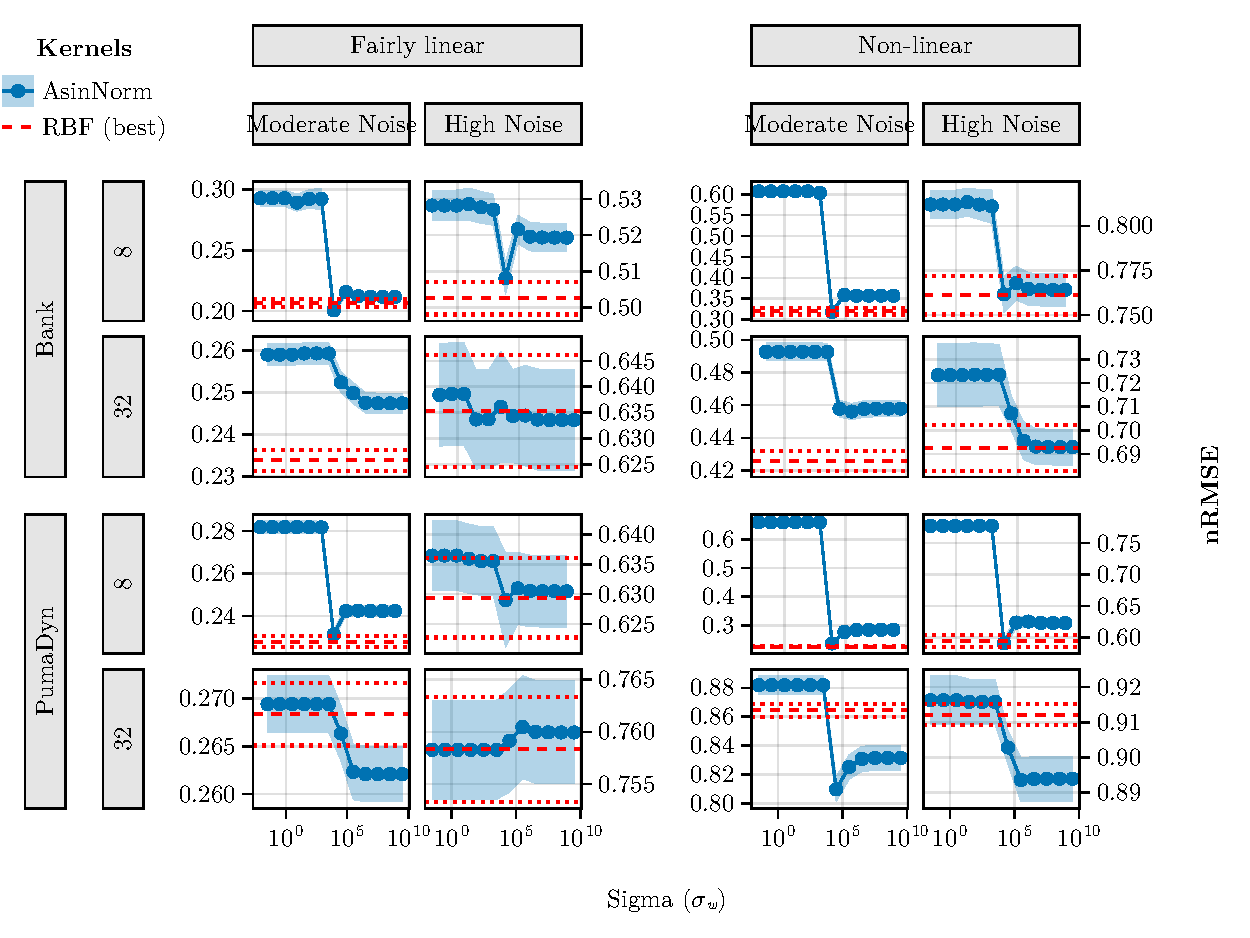
\includegraphics[width=\textwidth,height=0.95\textheight]{./figures/plots/nRMSE_delve_asinnorm_scaled_unlinked}
	\end{figure}
\end{frame}

% \begin{frame}{Results \textendash{} Normalized Arcsine kernel and RBF \textendash{} $t$\textendash{}test}
% 	\begin{columns}
% 		\begin{column}{0.47\textwidth}
% 			\begin{figure}[H]
% 				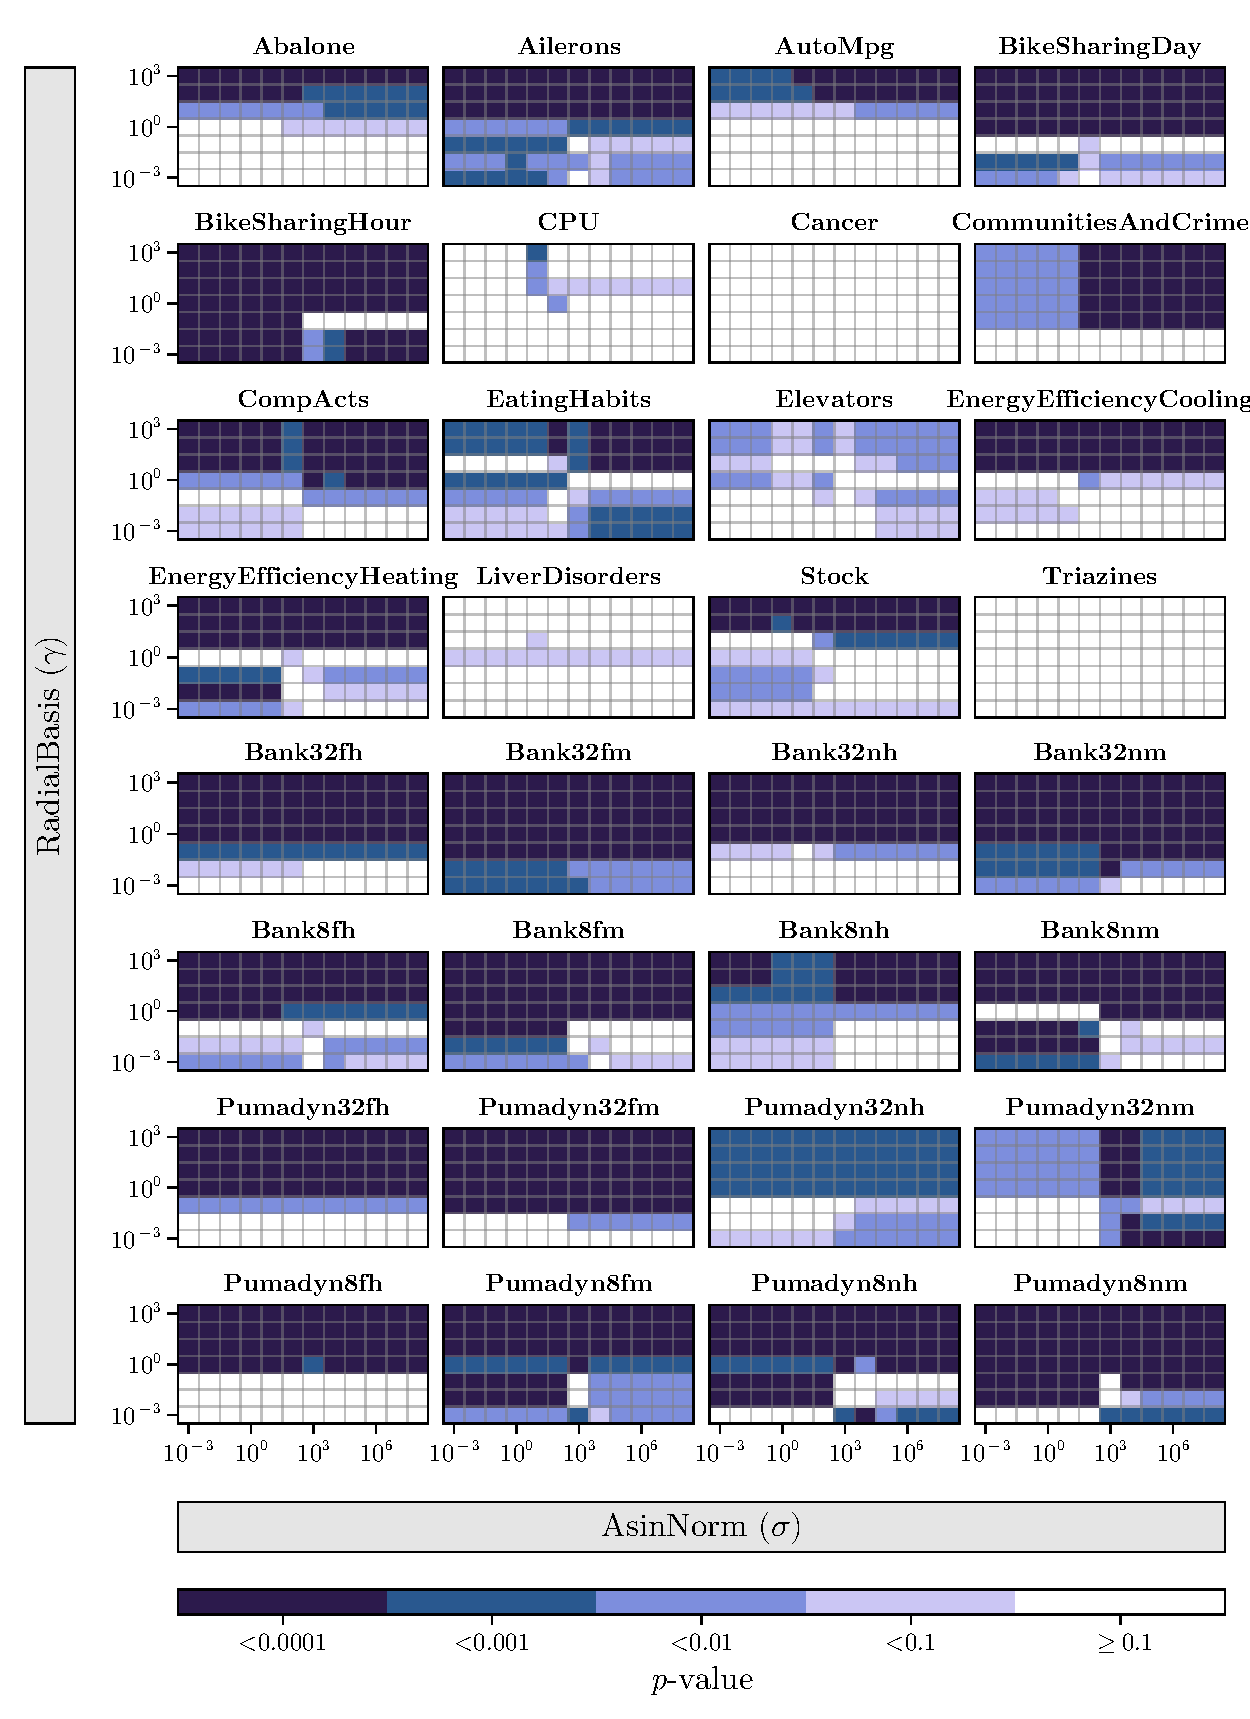
\includegraphics[width=\textwidth,height=0.95\textheight]{./figures/plots/heatmaps_rbf_asinnorm_pvalues}
% 			\end{figure}
% 		\end{column}
% 		\textrightarrow{}
% 		\begin{column}{0.47\textwidth}
% 			\begin{figure}[H]
% 				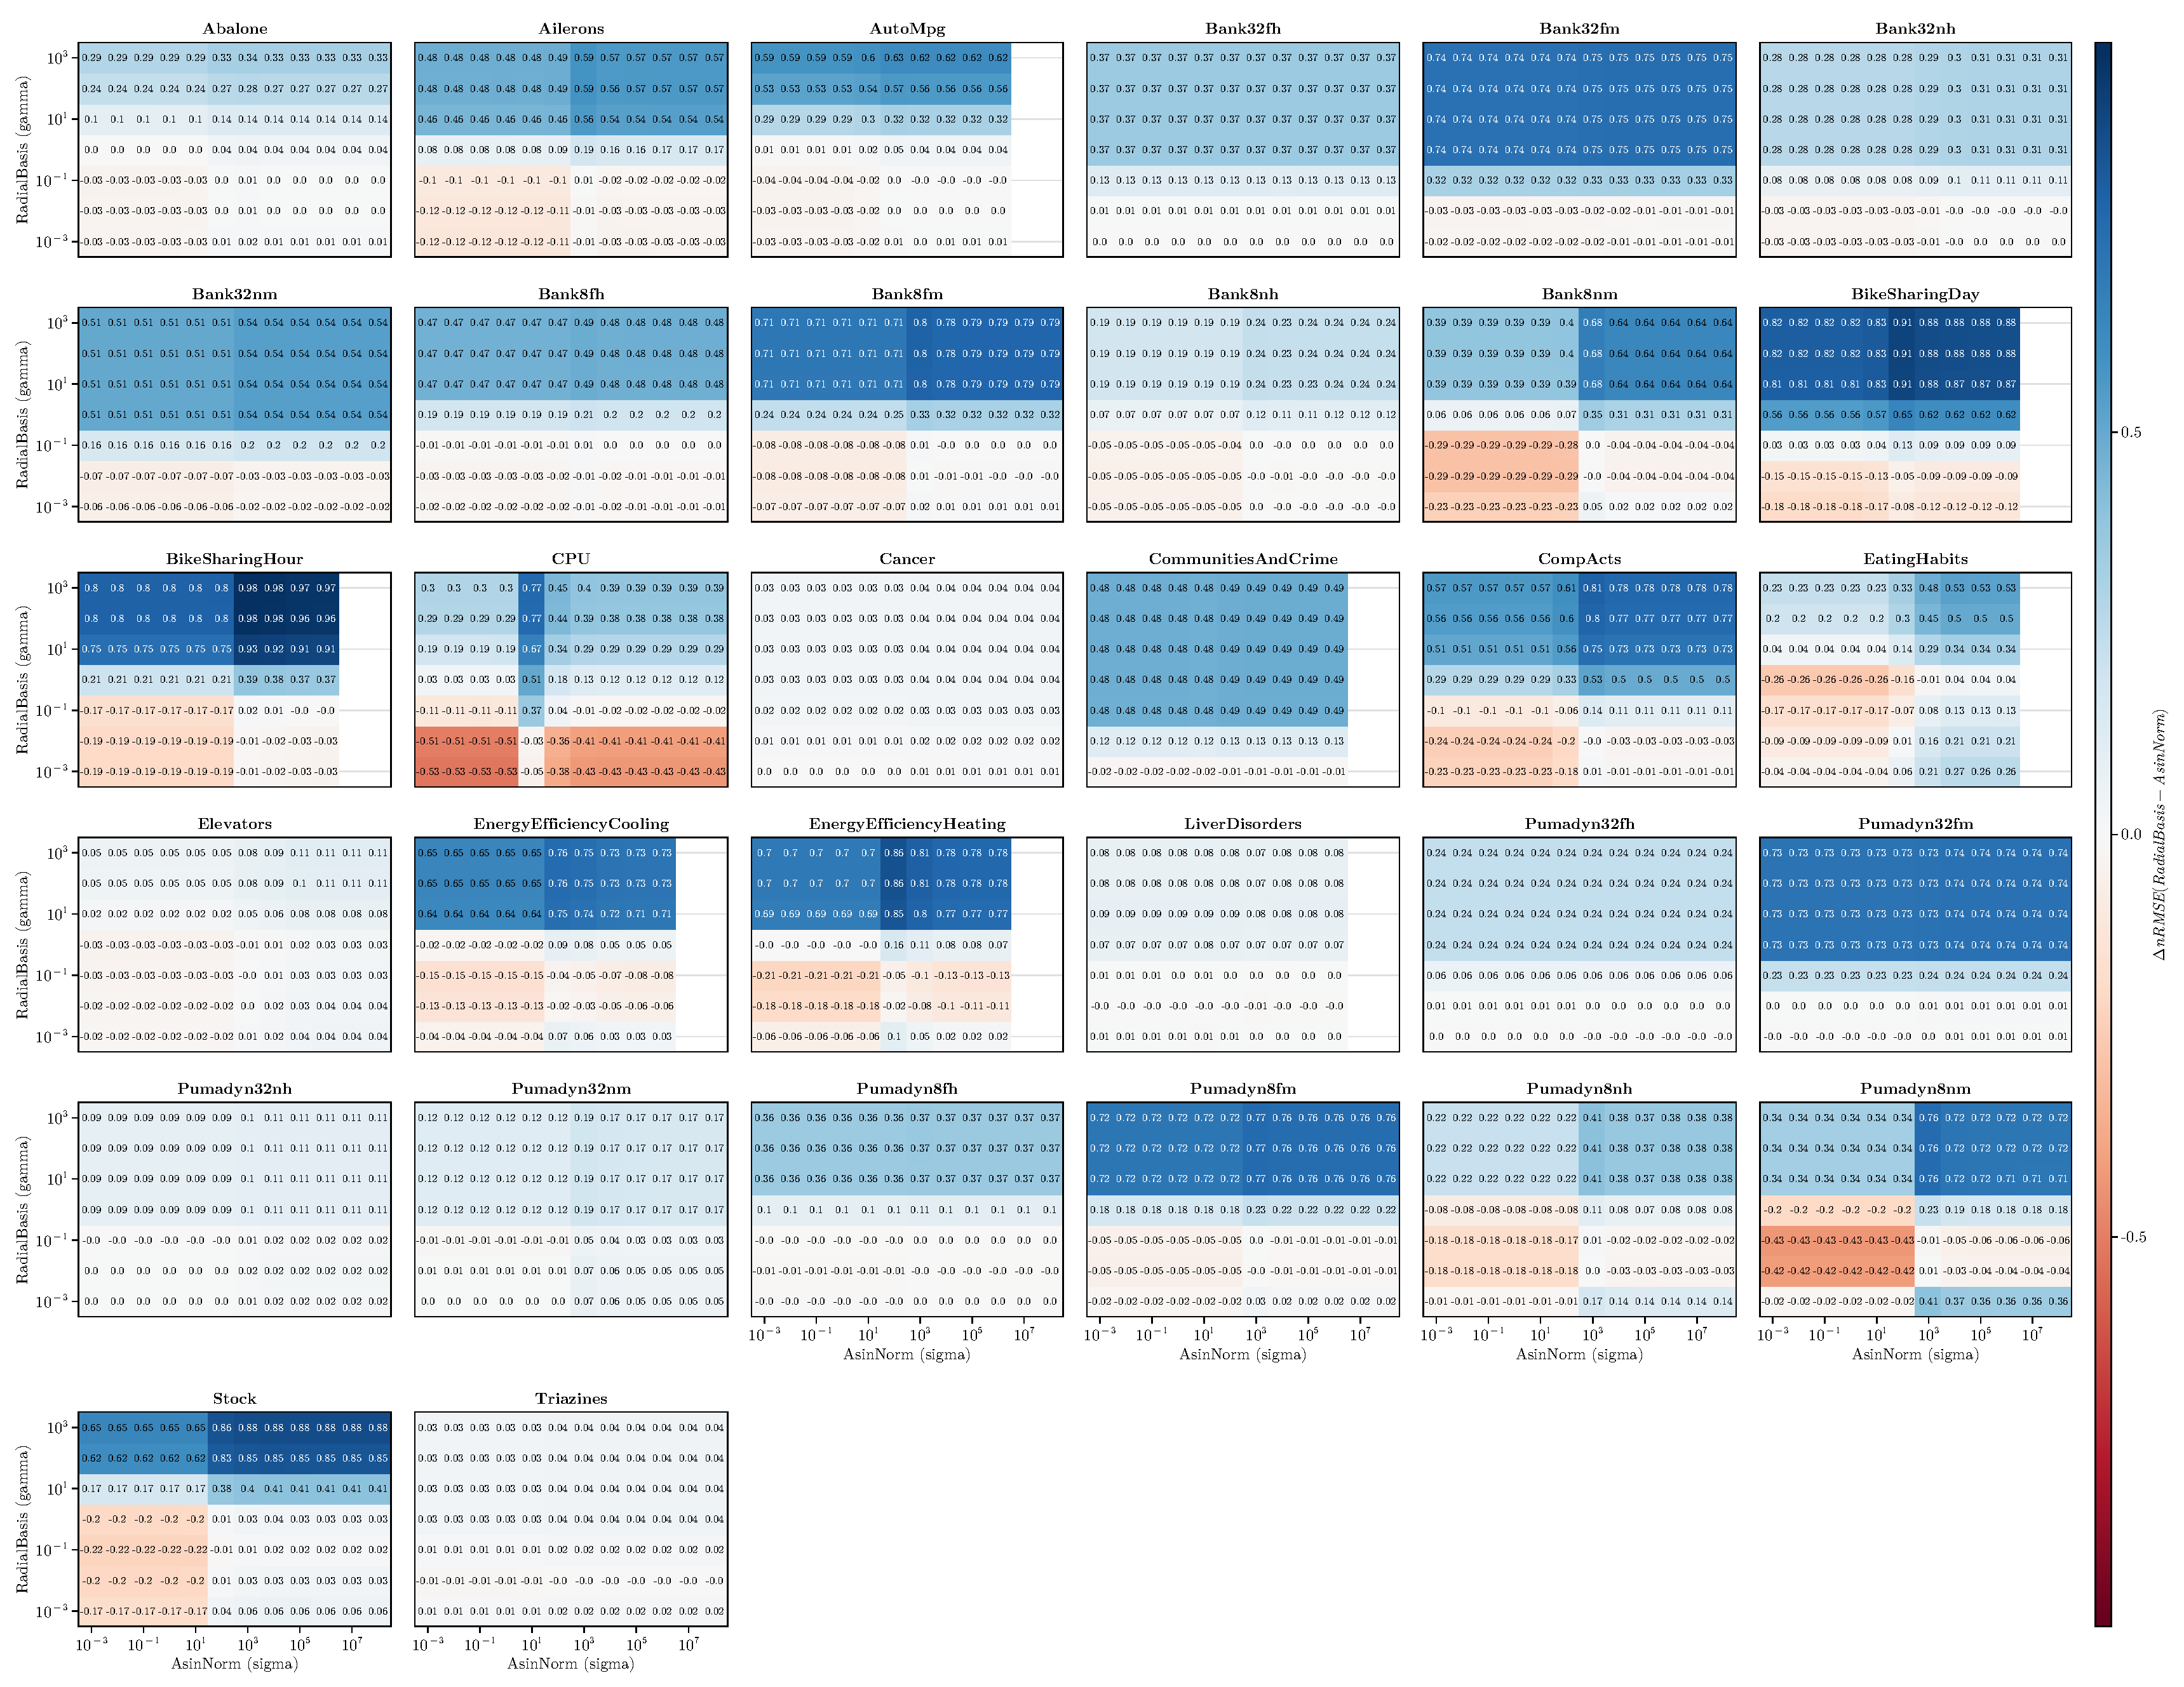
\includegraphics[width=\textwidth,height=0.95\textheight]{./figures/plots/heatmaps_rbf_asinnorm}
% 			\end{figure}
% 		\end{column}
% 	\end{columns}
% \end{frame}

\begin{frame}{Results \textendash{} Normalized Arcsine kernel and RBF \textendash{} $t$\textendash{}test}
	\centering $p$\textendash{}values
	\begin{figure}[H]
		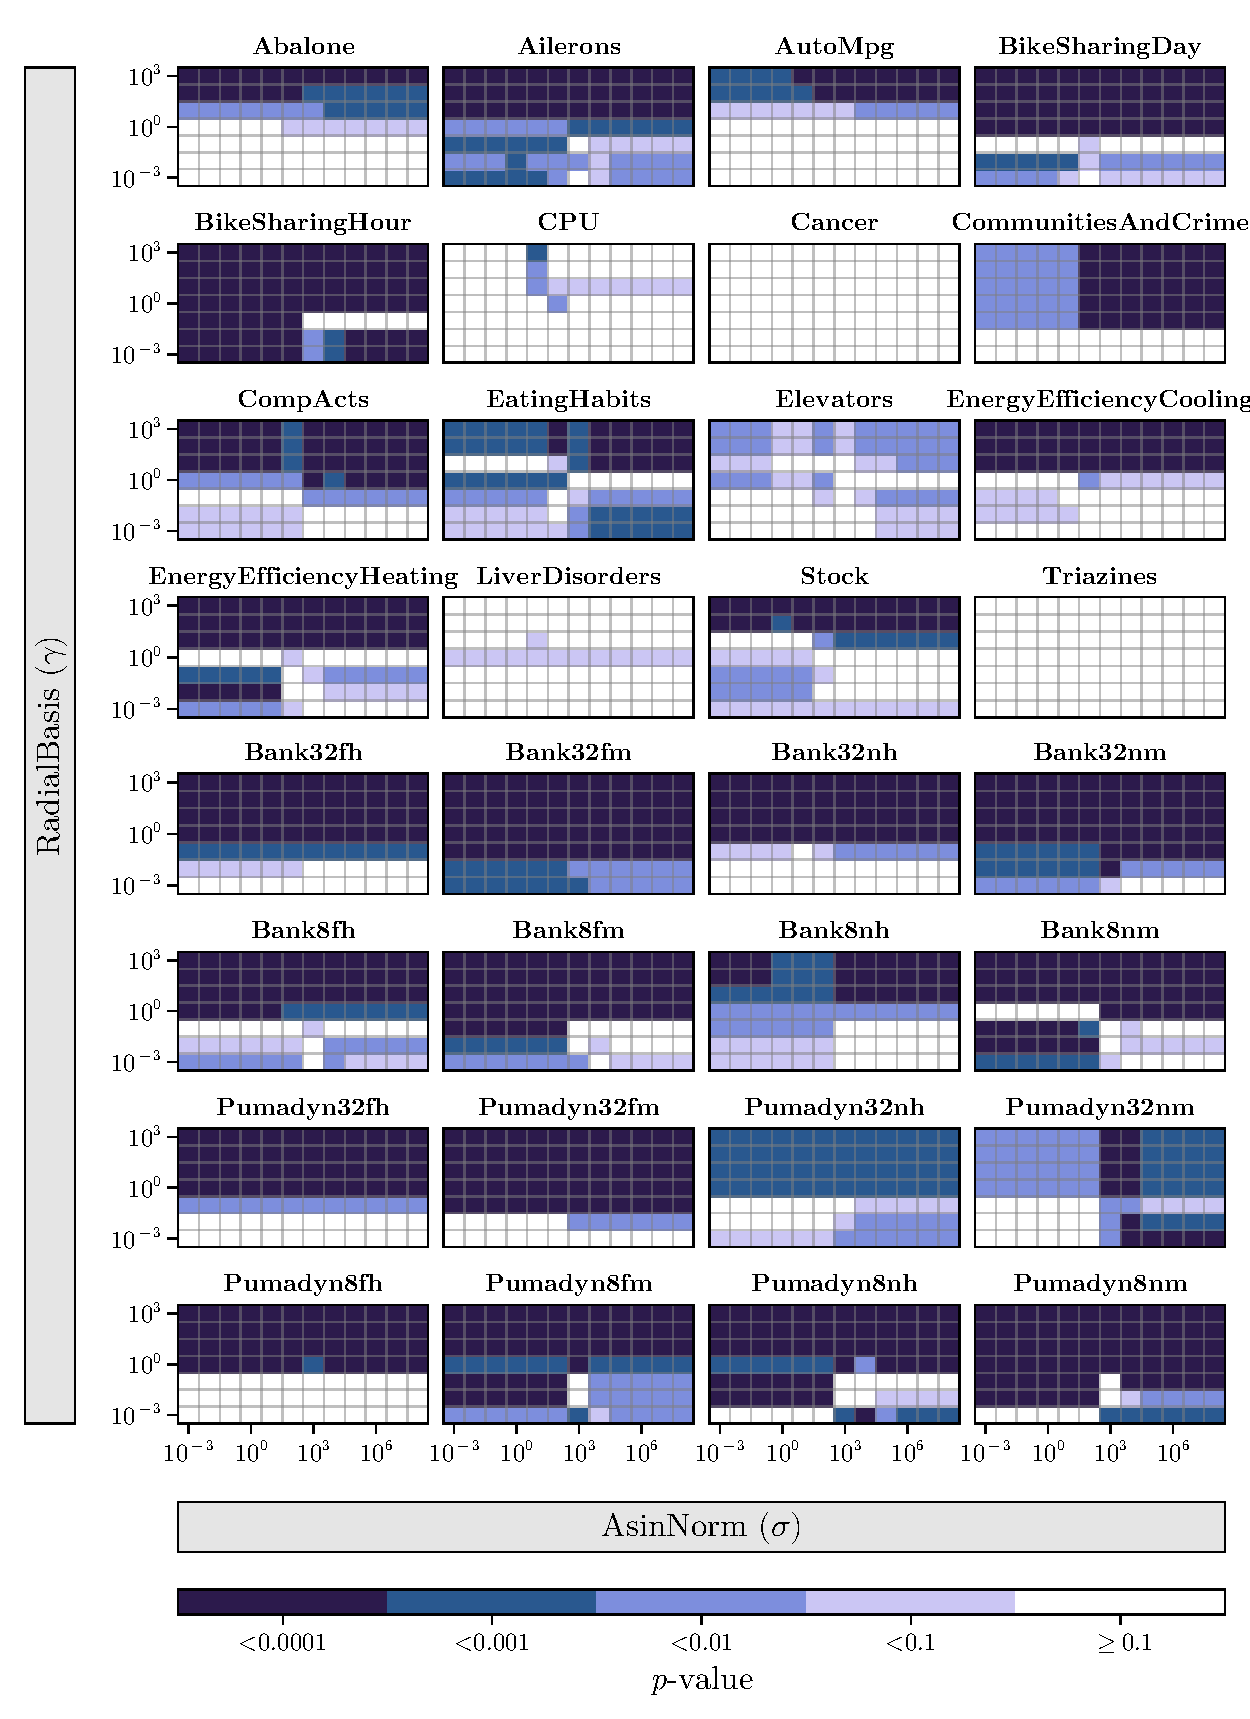
\includegraphics[width=\textwidth,height=0.85\textheight]{./figures/plots/heatmaps_rbf_asinnorm_pvalues}
	\end{figure}
\end{frame}
\note[itemize] {
	\item The lower the p values, the more significant the difference in performance.
}

\begin{frame}{Results \textendash{} Normalized Arcsine kernel and RBF \textendash{} $t$\textendash{}test}
	\centering Difference in performance
	\begin{figure}[H]
		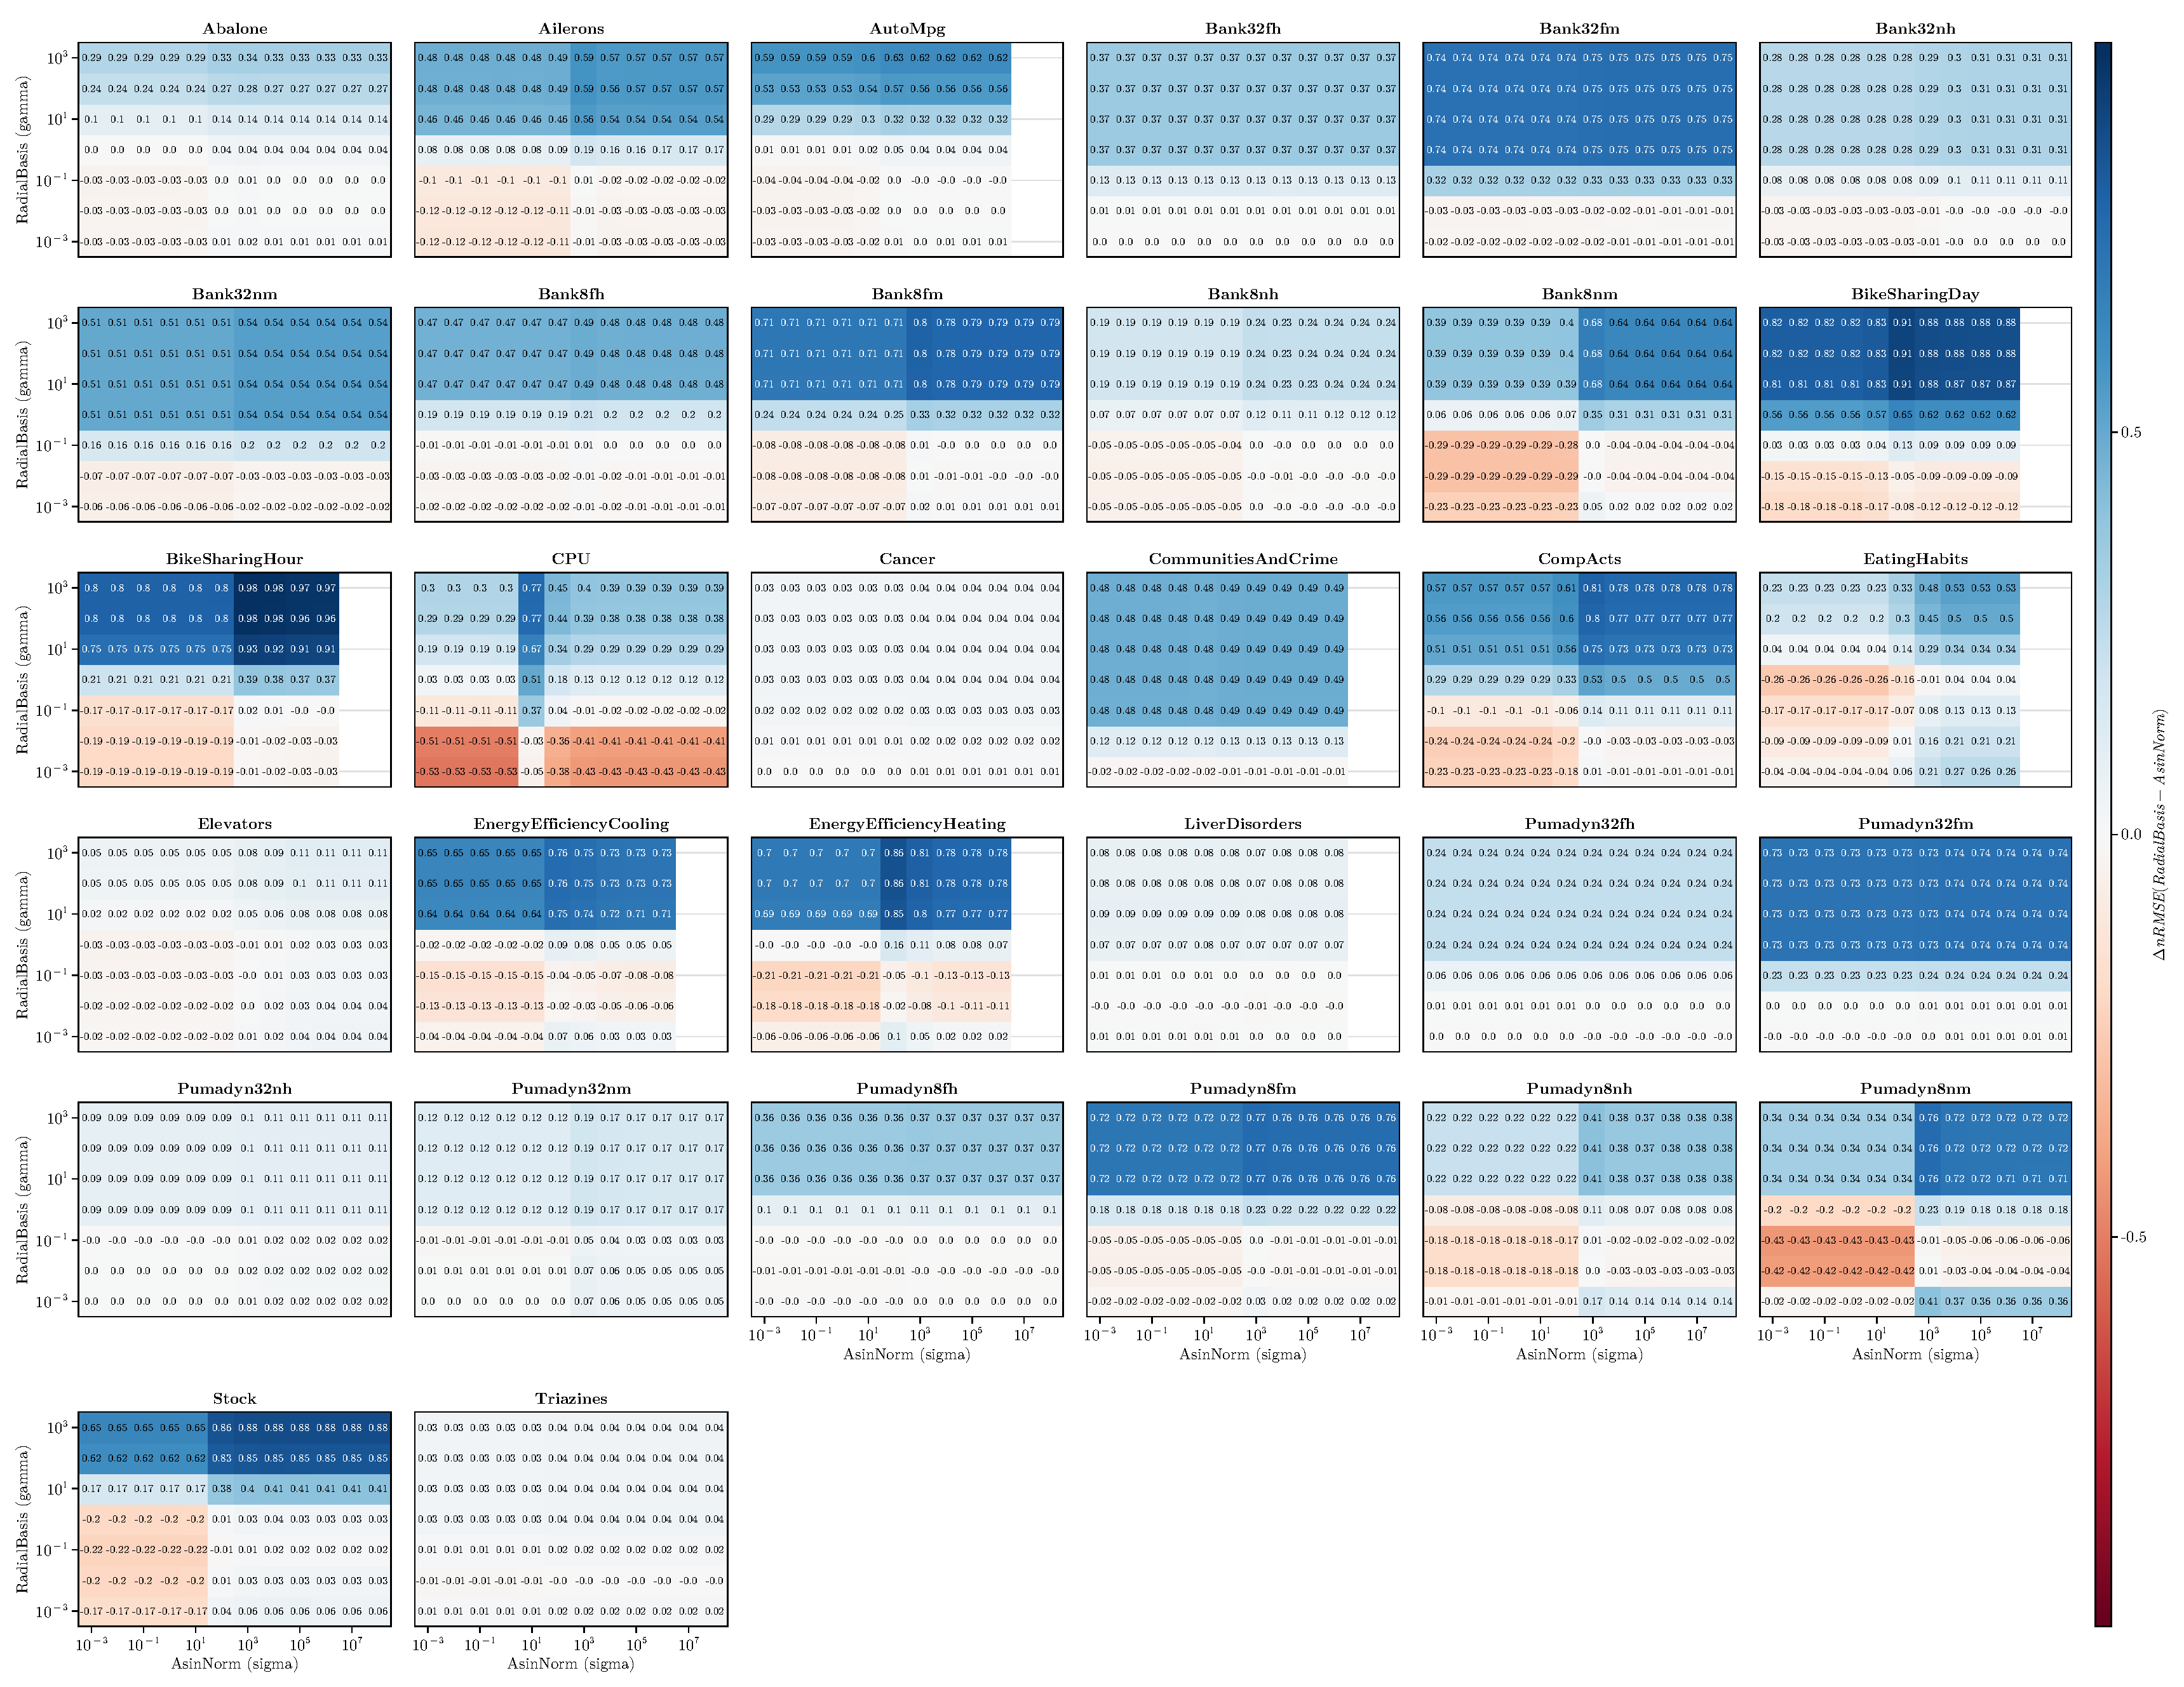
\includegraphics[width=\textwidth,height=0.85\textheight]{./figures/plots/heatmaps_rbf_asinnorm}
	\end{figure}
\end{frame}
\note[itemize] {
	\item Red means that the RBF kernel is better than the arcsine kernel.
	\item Blue means that the arcsine kernel is better than the RBF kernel.
}


\begin{frame}{Results \textendash{} Effects of normalization on Arcsine kernel}
	\begin{figure}[H]
		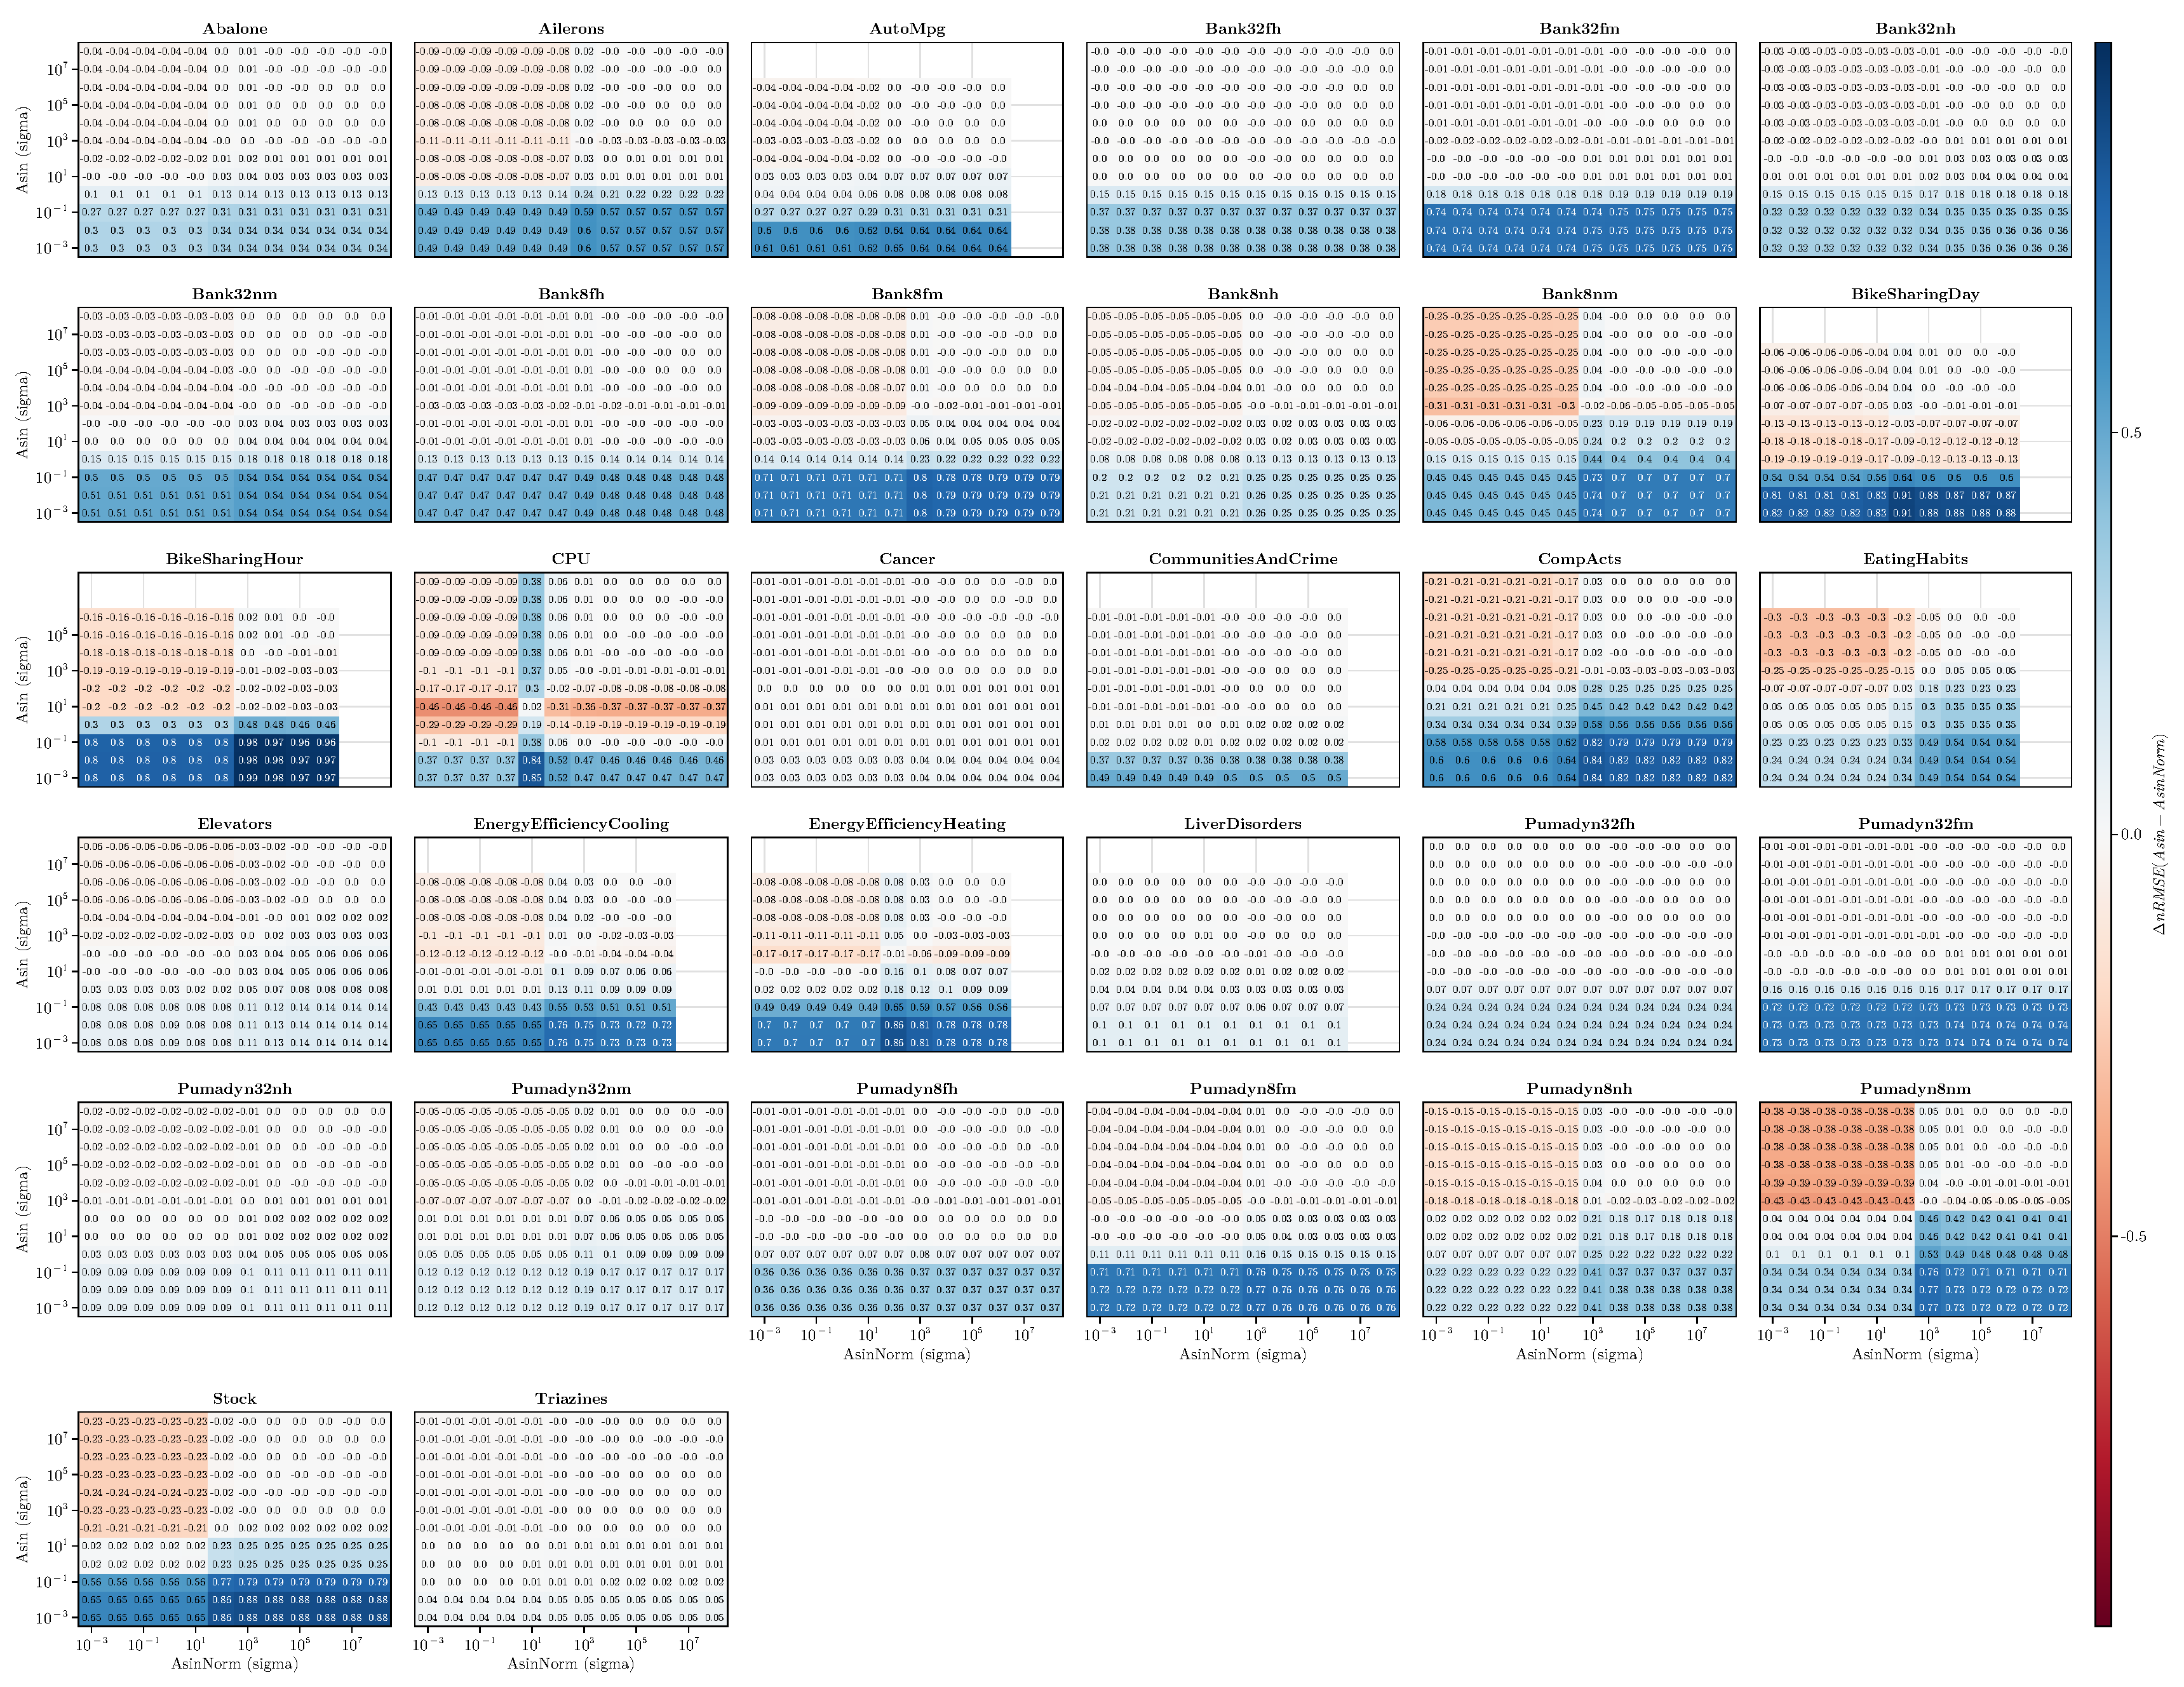
\includegraphics[width=\textwidth,height=0.95\textheight]{./figures/plots/heatmaps_asin_asinnorm}
	\end{figure}
\end{frame}
\note[itemize]{
	\item $p$-values omitted
	\item The performance of the normalized arcsine kernel is equivalent to the non-normalized arcsine kernel when
	both sigmas are large. (Top right corner)
}

% \begin{frame}{Results \textendash{} Normalized Arccosine kernels}
% 	% \begin{figure}[H]
% 	%     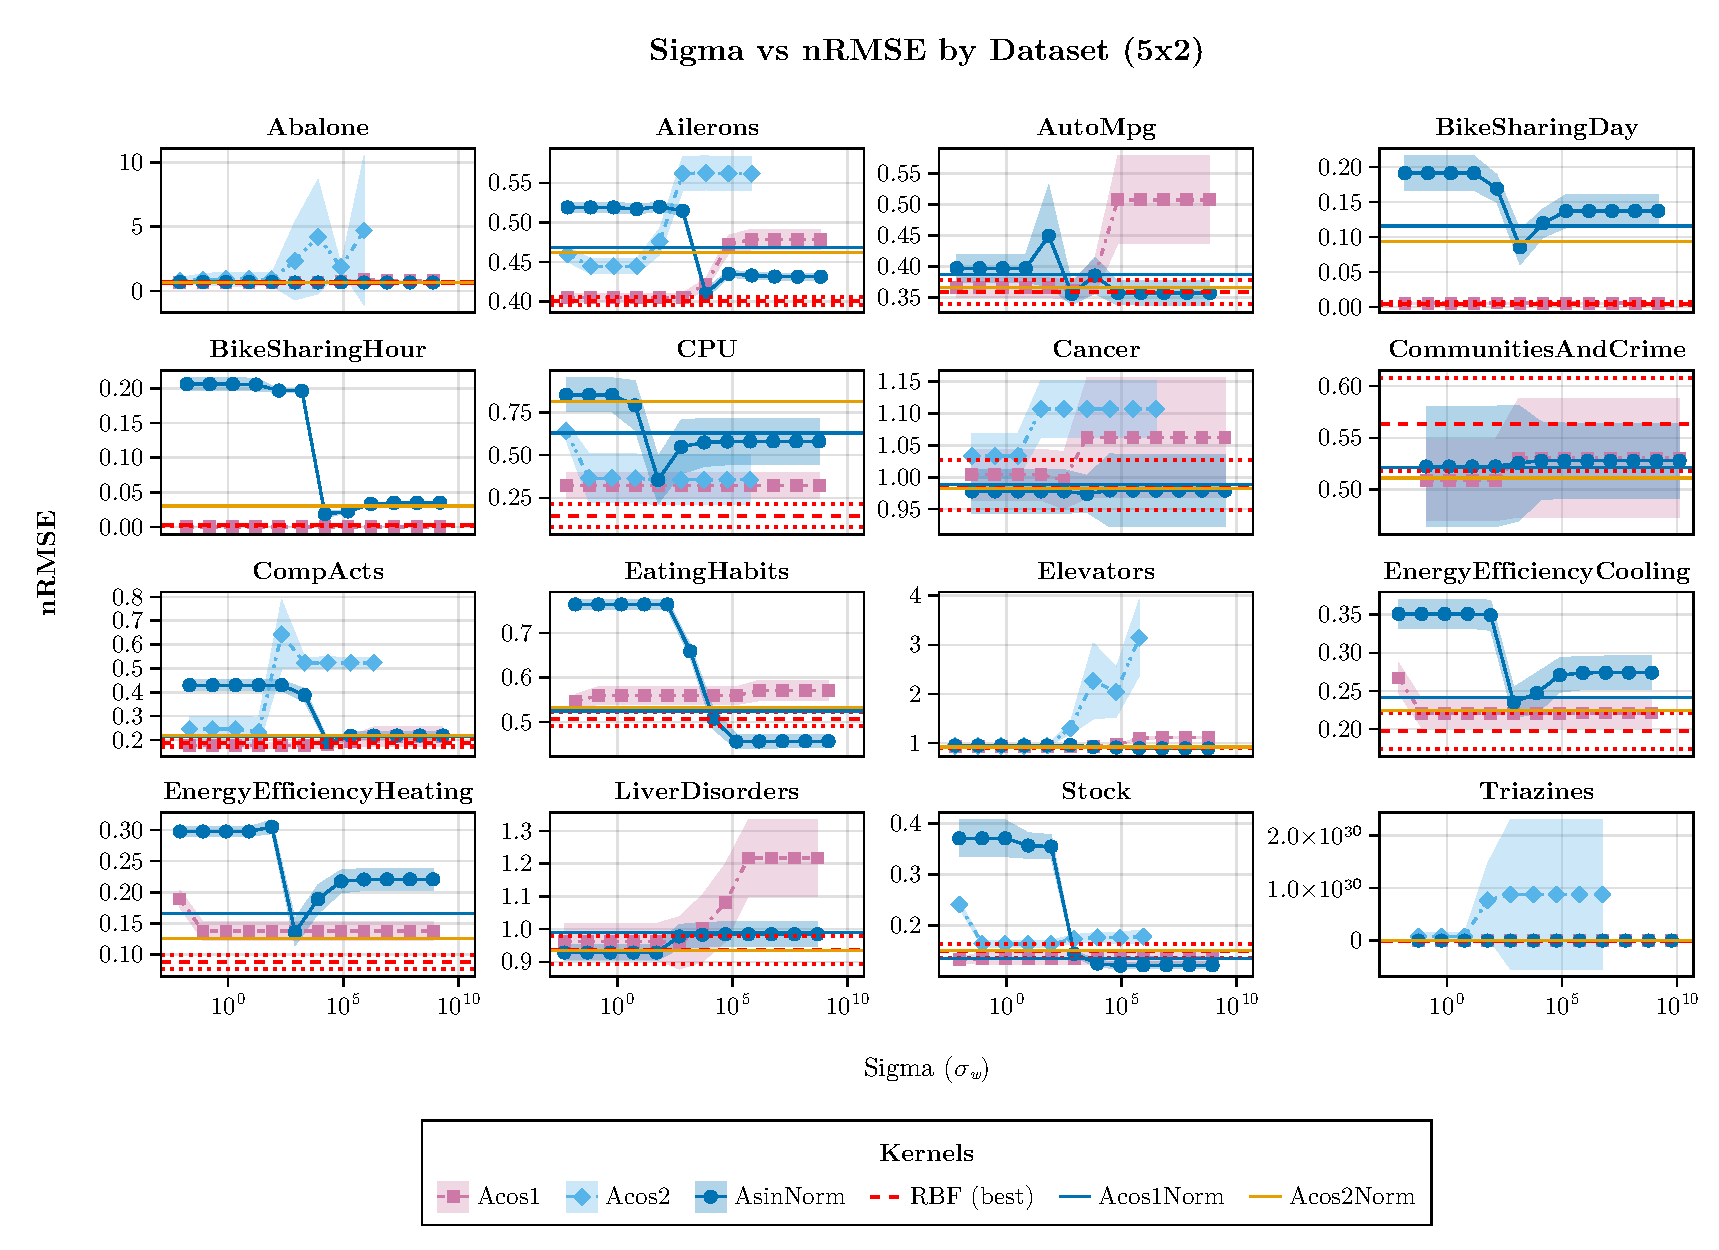
\includegraphics[width=\textwidth,height=0.95\textheight]{./figures/plots/nRMSE_nodelve_acos_scaled}
% 	% \end{figure}
% \end{frame}

\begin{frame}{Results \textendash{} Arccosine kernels}
	\begin{figure}[H]
		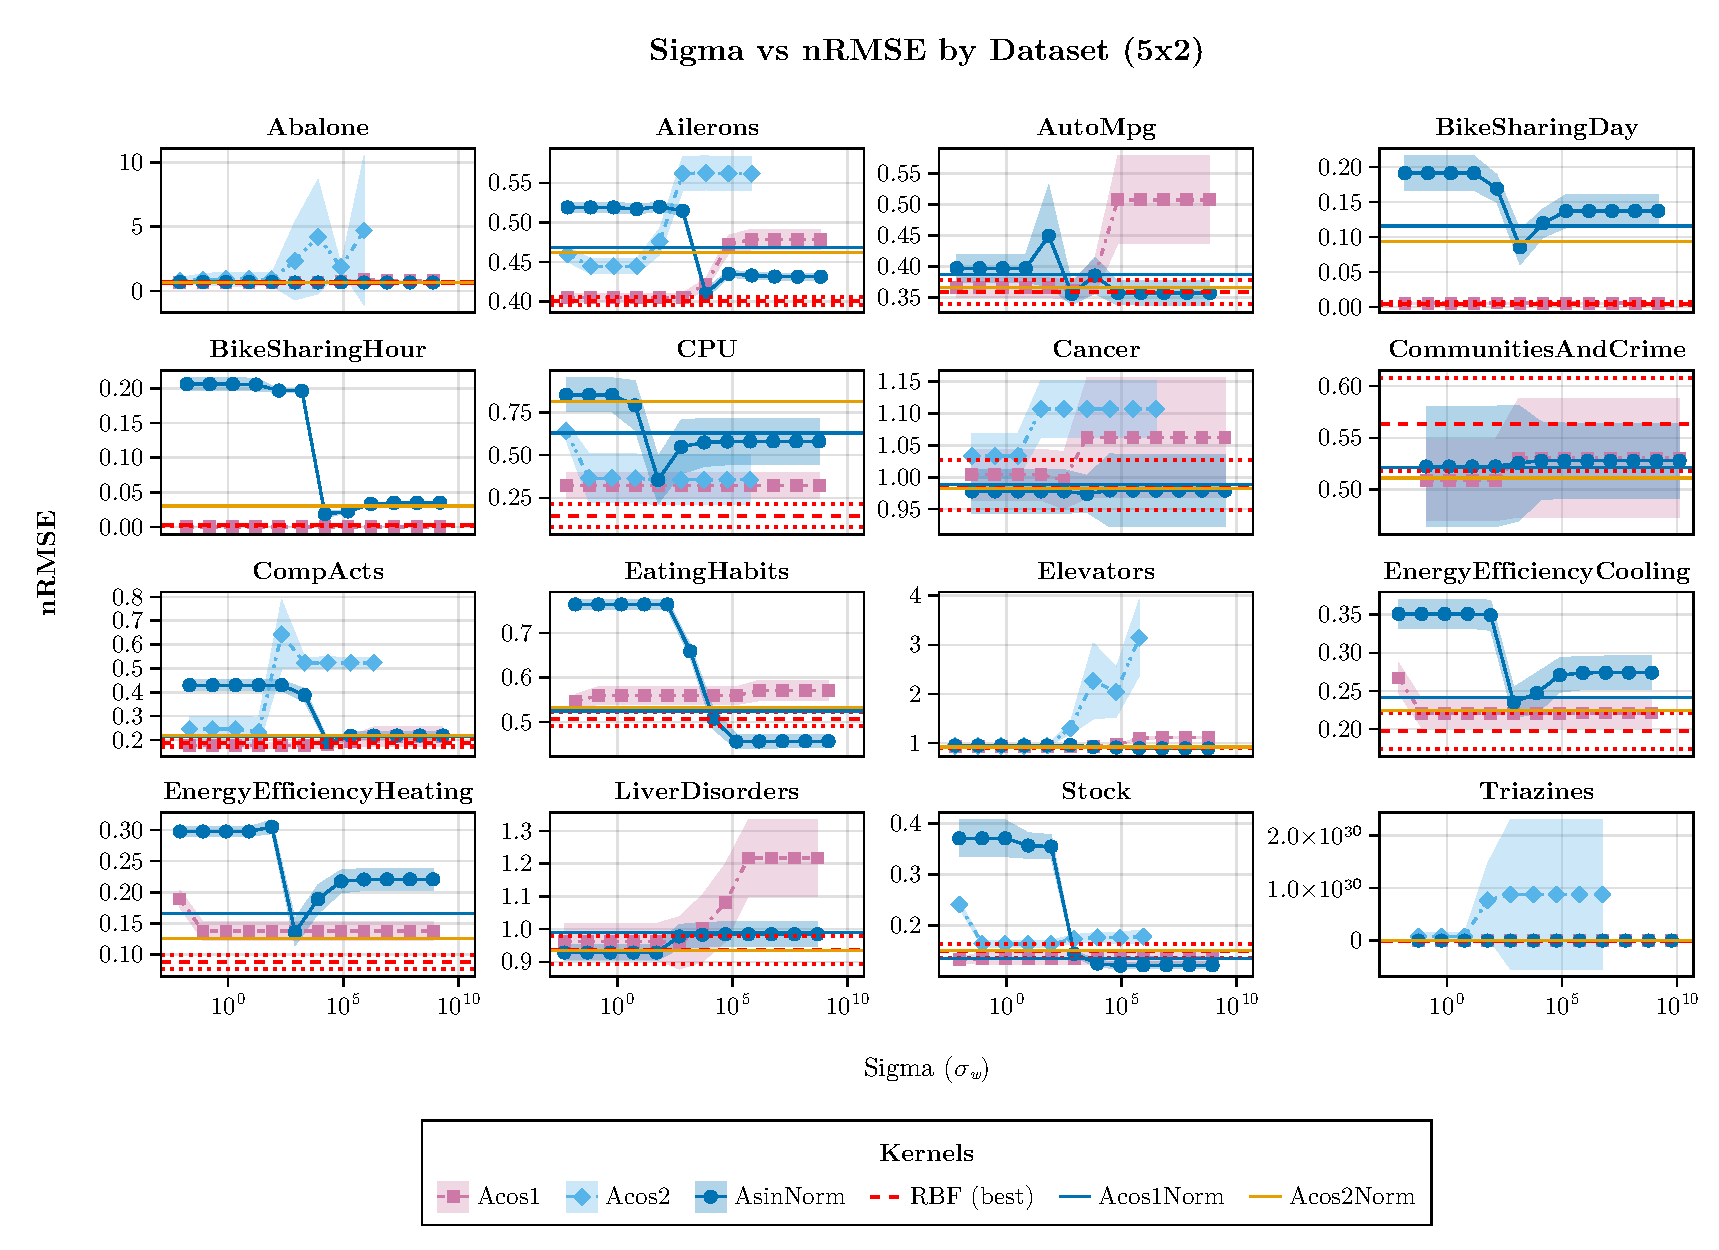
\includegraphics[width=\textwidth,height=0.95\textheight]{./figures/plots/nRMSE_nodelve_acos_scaled}
	\end{figure}
\end{frame}

\begin{frame}{Results \textendash{} Numerical issues with arccosine kernel}
	\begin{columns}
		\begin{column}{0.33\textwidth}
			\begin{figure}[H]
				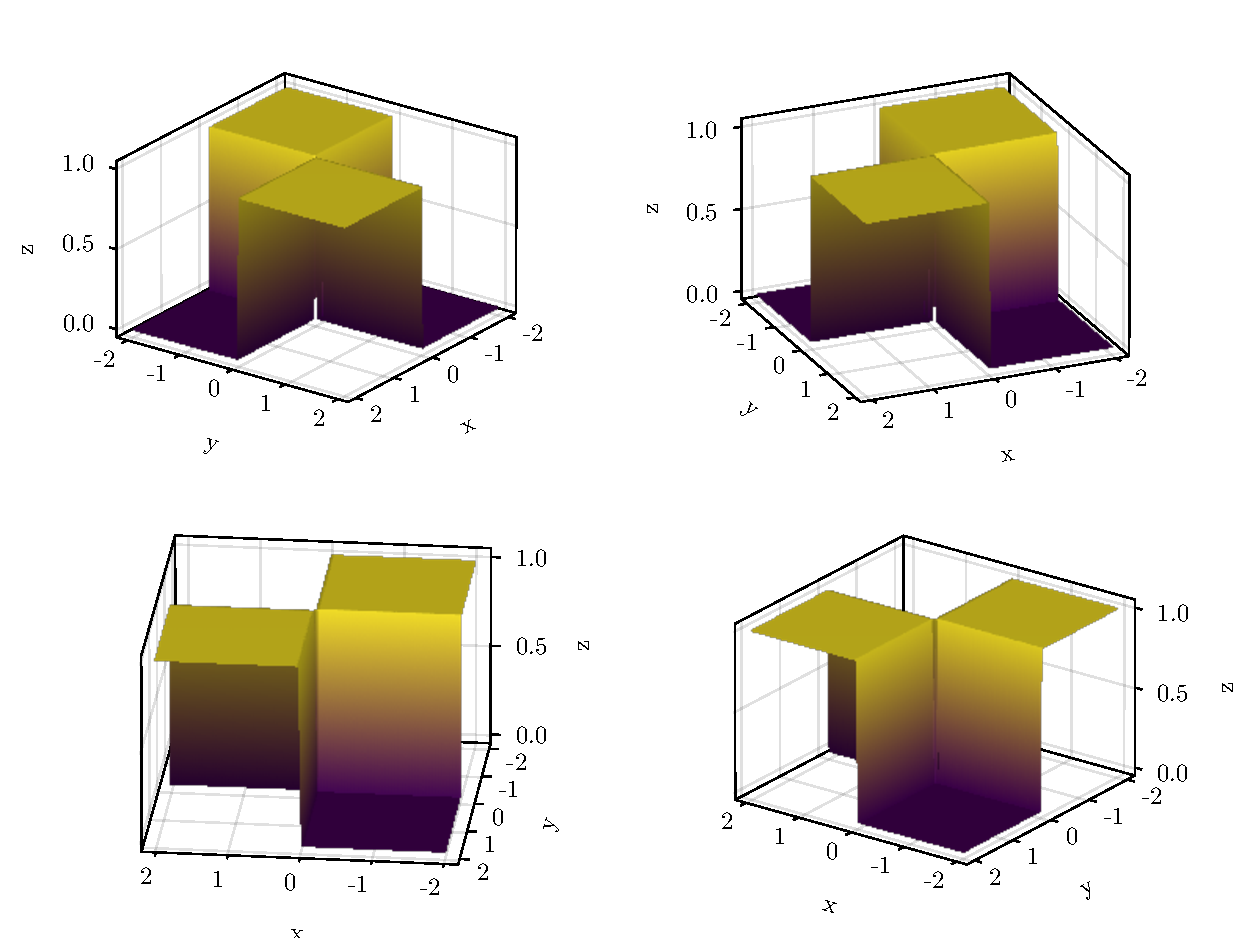
\includegraphics[width=\textwidth,height=0.95\textheight]{./figures/plots/kernel_acos0_3d.pdf}
				\caption*{Arccosine kernel for $n=0$}
			\end{figure}
		\end{column}
		\begin{column}{0.33\textwidth}
			\begin{figure}[H]
				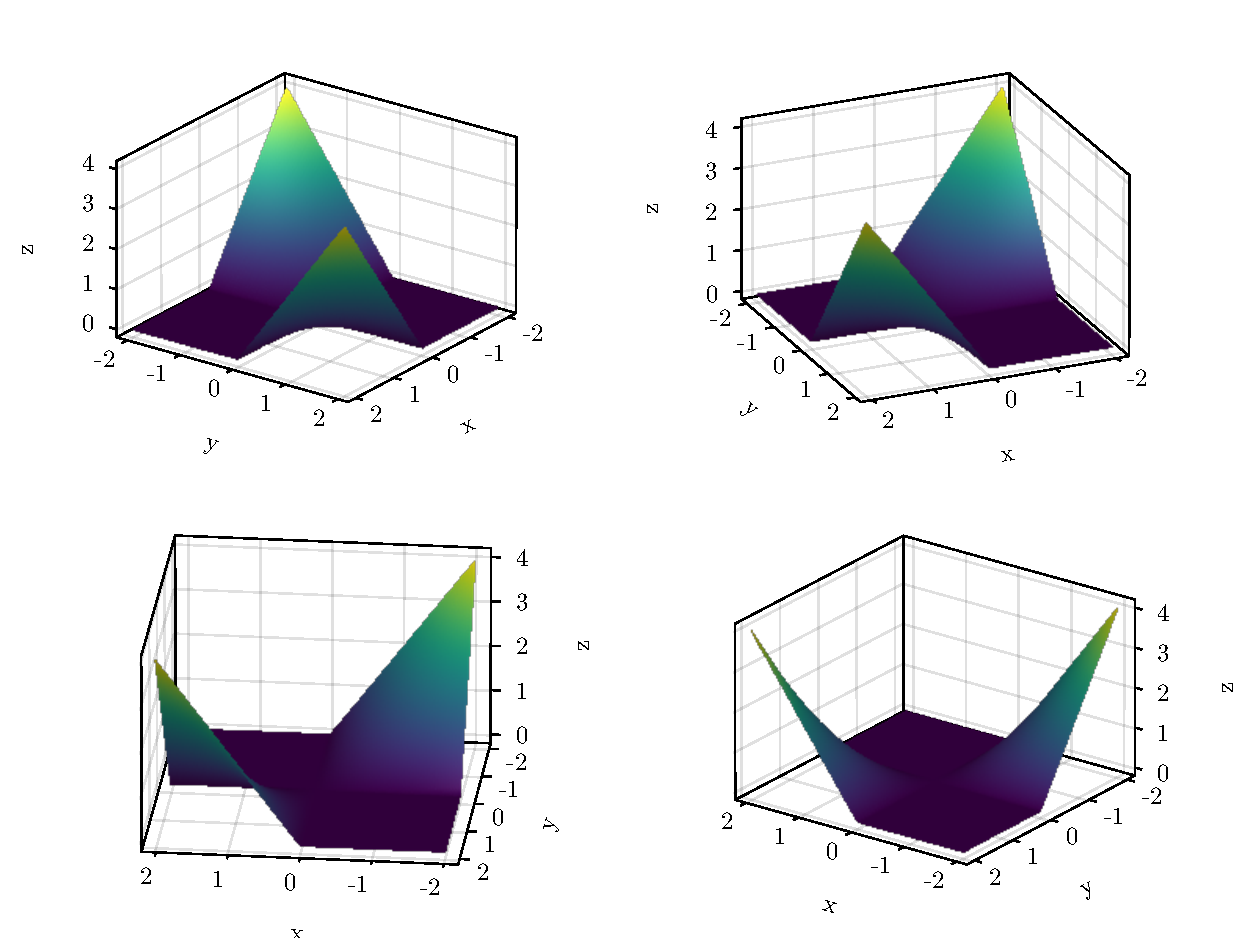
\includegraphics[width=\textwidth,height=0.95\textheight]{./figures/plots/kernel_acos1_3d.pdf}
				\caption*{Arccosine kernel for $n=1$}
			\end{figure}
		\end{column}
		\begin{column}{0.33\textwidth}
			\begin{figure}[H]
				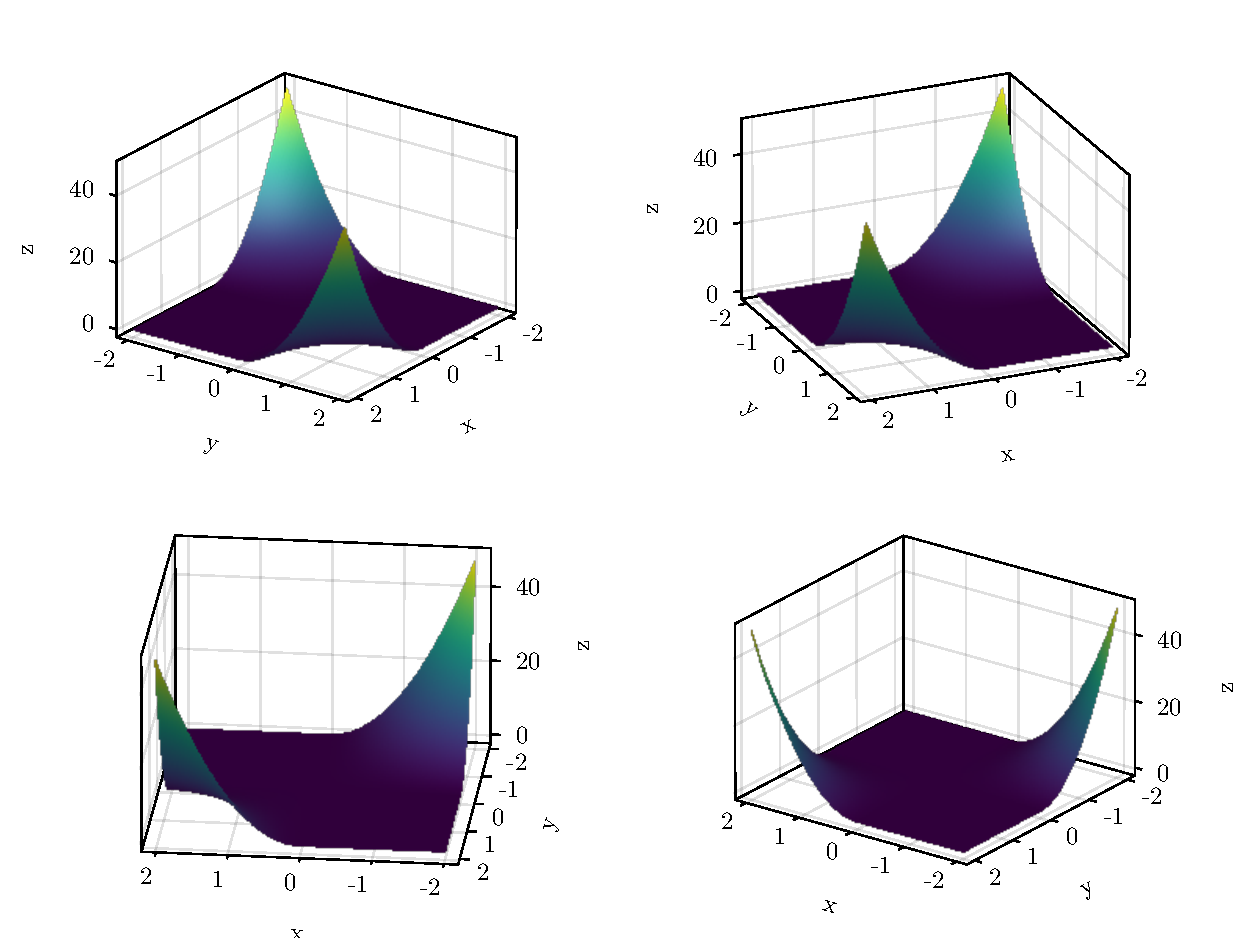
\includegraphics[width=\textwidth,height=0.95\textheight]{./figures/plots/kernel_acos2_3d.pdf}
				\caption*{Arccosine kernel for $n=2$}
			\end{figure}
		\end{column}
	\end{columns}
\end{frame}

\begin{frame}{Results \textendash{} Arccosine kernel $n=1$}
	\begin{figure}[H]
		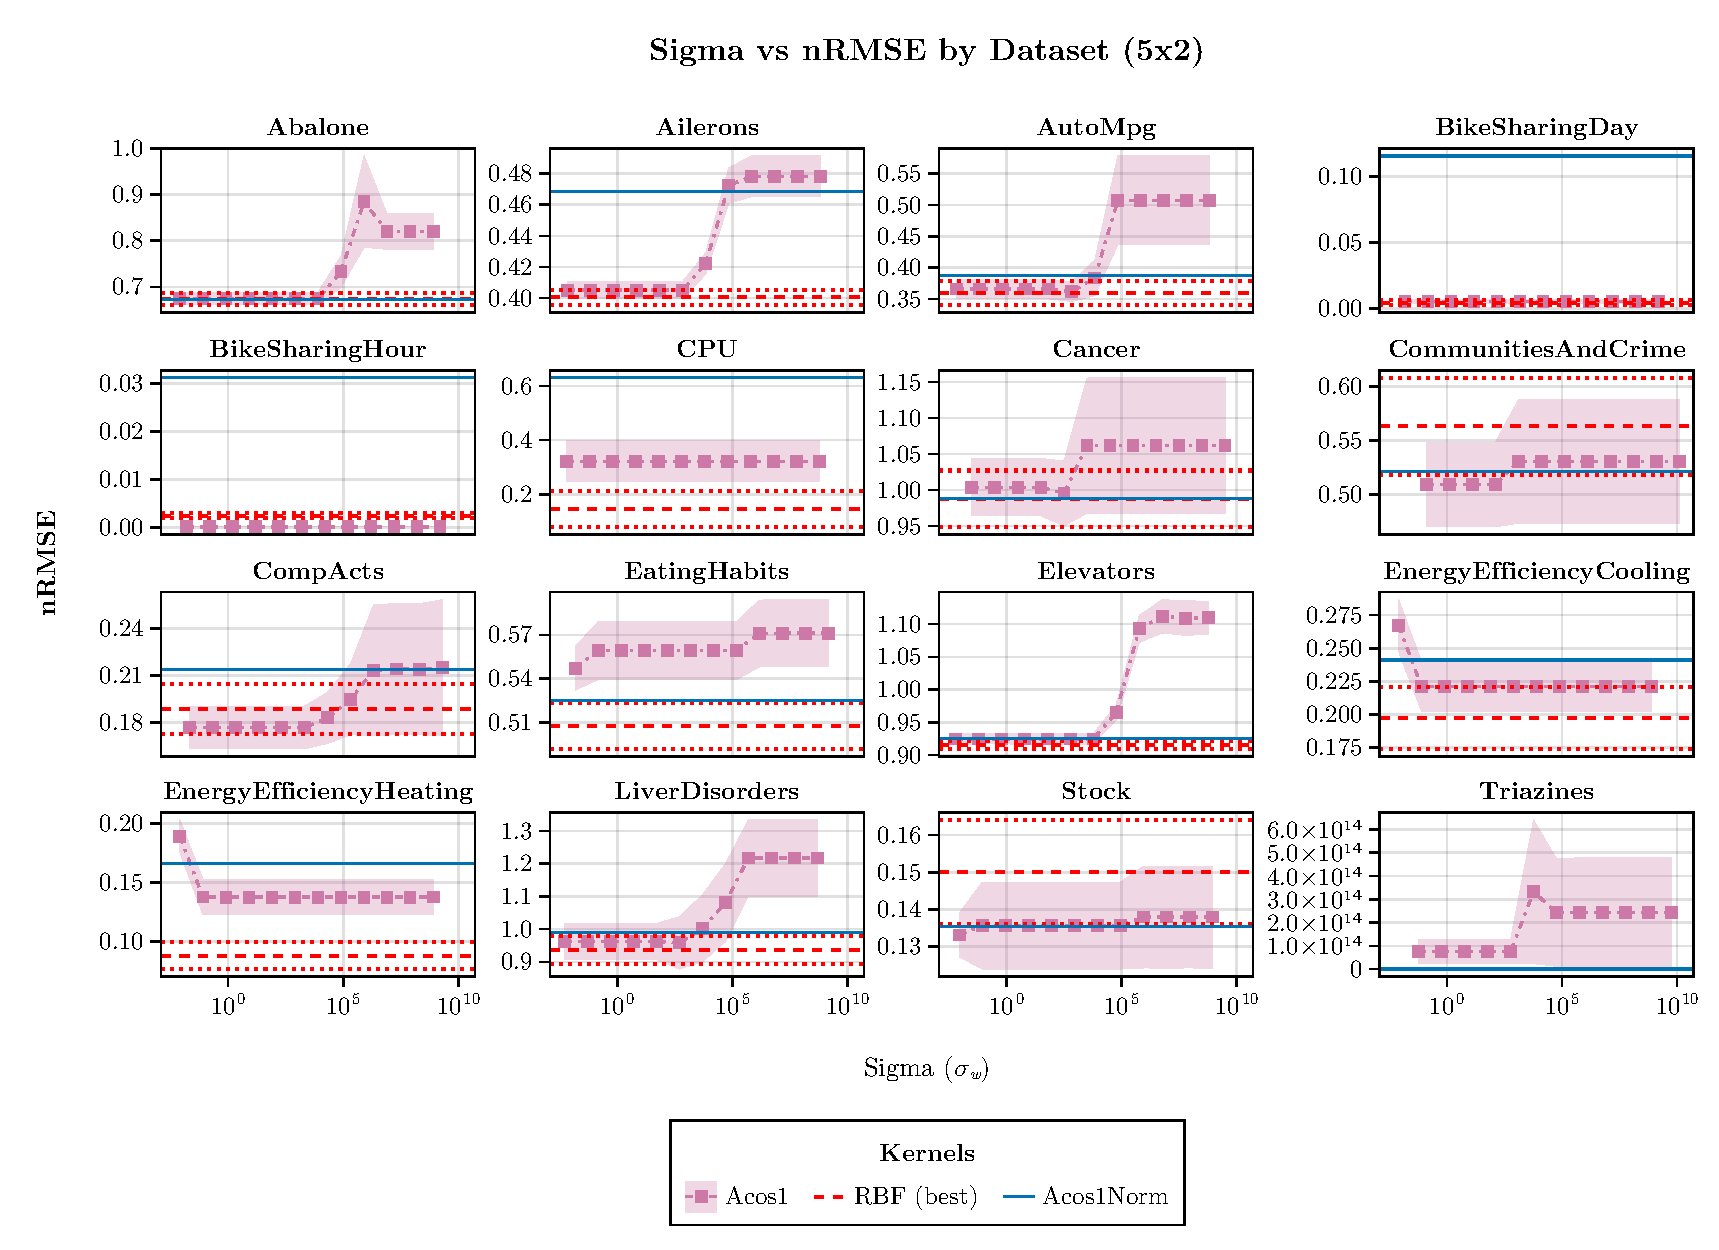
\includegraphics[width=\textwidth,height=0.95\textheight]{./figures/plots/nRMSE_nodelve_acos1_scaled}
	\end{figure}
\end{frame}
\note[itemize]{
	\item Still some issues in Triazines and LiverDisorders.
}

\section{Conclusions}

\begin{frame}{Conclusions}
	\begin{itemize}%[<+->]
		\item Both the arcsine and arccosine kernels show \emph{parameter-insensitive} behaviour.
		\item For large values of $\sigma$ the performance of the arcsine kernel is
		      comparable to the Gaussian kernel.
		\item For large values of $\sigma$, in normalized data, the performance
		      of the normalized arcsine and non-normalized arcsine kernels is equivalent.
		\item Arcsine kernel reaches parity with the RBF kernel, but not necessarily
		      when $\sigma$ is large.
		\item The arccosine kernel is numerically unstable for $n>0$ when not
		      normalized.
	\end{itemize}
\end{frame}

\begin{frame}{Further Work}
	\begin{itemize}
		\item Increase significantly the number of datasets.
		\item Investigate the behaviour of the arccosine kernel for $n>2$.
	\end{itemize}
\end{frame}

\begin{frame}[standout]
	Thank you!
\end{frame}

\begin{frame}{Outline}
	\vspace{1em}
	\setcounter{tocdepth}{1}
	\tableofcontents
\end{frame}
% Add extra slides for presentation
\appendix

%bibilio
\begin{frame}[allowframebreaks]{References}
	\printbibliography[heading=none]
\end{frame}

\begin{frame}[standout]
	Bonus slides
\end{frame}

\begin{frame}{Cross validation in \textcite{frenayParameterinsensitiveKernelExtreme2011}}
	\begin{figure}[H]
		\resizebox{0.95\textwidth}{0.9\textheight}{
			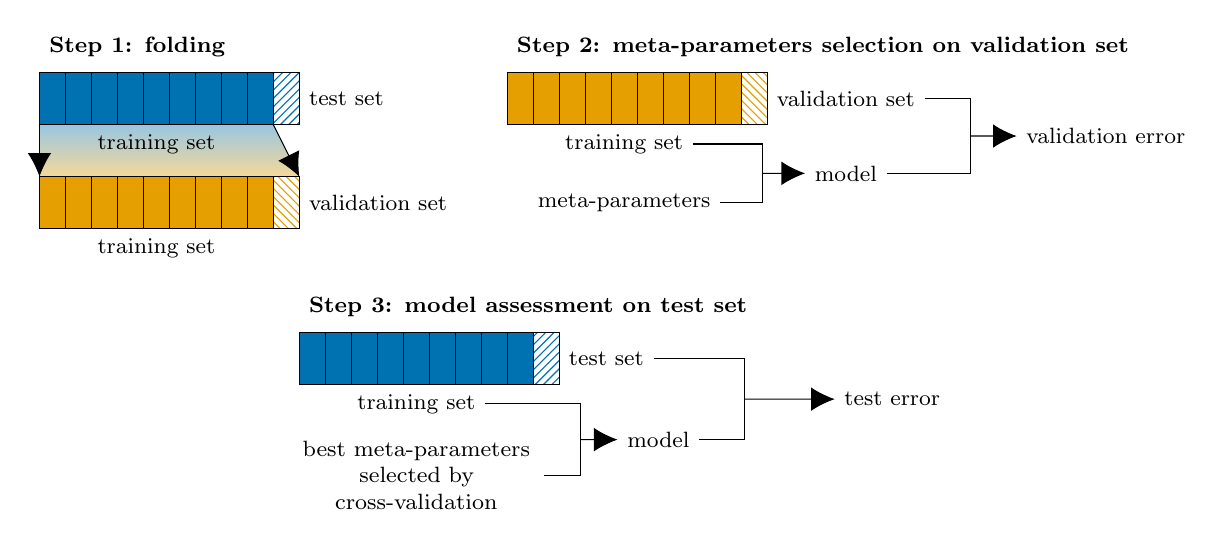
\begin{tikzpicture}[
		scale=0.66,
		every node/.style={font=\footnotesize},
	]
	% Draw main rectangle
	\def\nfolds{10}
	\pgfmathsetmacro{\trainfolds}{\nfolds-1}
	\pgfmathsetmacro{\splits}{\nfolds-2}
	\def\heightmult{0.5}

	\newcommand{\fold}[5]{%
		\draw[#2] #1 rectangle ($#1+(\heightmult*\trainfolds,1)$);
		% fill with pattern
		\filldraw[#3] ($#1+(\heightmult*\trainfolds,0)$) rectangle ($#1+(\heightmult*\nfolds,1)$);

		\draw ($#1+(\heightmult*\trainfolds/2,0)$) node[below,name=below-#5] {training set};
		\draw ($#1+(\heightmult*\nfolds,0.5)$) node[right,name=right-#5] {#4 set};

		% Draw vertical dashed lines for fold divisions
		\foreach \x in {1,...,\splits}{
				\draw ($#1+(\heightmult*\x,0)$) -- ($#1+({\heightmult*\x},1)$);
			}
	}

	\def\coltest{wong_blue}
	\def\colvali{wong_orange}

	\fill[shading=axis,top color=\coltest!40,bottom color=\colvali!40] (0,0) -- (\heightmult*\trainfolds,0) -- (\heightmult*\nfolds,-1) -- (0,-1) -- cycle;

	\fold{(0,0)}{fill=\coltest}{pattern=north east lines, pattern color=\coltest}{test}{test1}
	\fold{(0,-2)}{fill=\colvali}{pattern=north west lines,pattern color=\colvali}{validation}{val1}

	\draw[->] (0,0) -- (0,-1);
	\draw[->] (\heightmult*\trainfolds,0) -- (\heightmult*\nfolds,-1);

	% title above bounding box
	% \draw (current bounding box.north) node[above] {\textbf{Step 1: folding}};

	\fold{(9,0)}{fill=\colvali}{pattern=north west lines,pattern color=\colvali}{validation}{val2}

	\draw (right-val1.east -| below-val2.south) node[name=meta-parameters] {meta-parameters};
	\coordinate (a) at ($(meta-parameters)!.5!(below-val2)$);
	\node[name=model] at (a -| right-val2) {model};

	\coordinate (vm) at ($(model)!.5!(right-val2)$);
	\node[name=valerr] at ($(vm)+(5,0)$) {validation error};

	\coordinate (mm) at ($(meta-parameters.east |- model.west)!0.5!(model.west)$);
	\draw (below-val2.east) -| (mm);
	\draw (meta-parameters.east) -| (mm);
	\draw[->] (mm) -- (model);

	\coordinate (vvm) at ($(right-val2.east |- valerr.west)!0.5!(valerr.west)$);
	\draw (right-val2.east) -| (vvm);
	\draw (model.east) -| (vvm);
	\draw[->] (vvm) -- (valerr);

	% step 3

	\coordinate (step3) at (5,-5);
	\fold{(step3)}{fill=\coltest}{pattern=north east lines,pattern color=\coltest}{test}{test3}

	\draw ($(below-test3.south)+(0,-1)$) node[name=best-meta-parameters,text width=3cm,align=center]
	{best meta-parameters selected by cross-validation};

	\coordinate (b) at ($(best-meta-parameters)!.5!(below-test3)$);
	\node[name=model3] at ($(b -| right-test3)+(1,0)$) {model};

	\coordinate (vm3) at ($(model3)!.5!(right-test3)$);
	\node[name=testerr] at ($(vm3)+(5,0)$) {test error};

	\coordinate (mm3) at ($(best-meta-parameters.east |- model3.west)!0.5!(model3.west)$);
	\draw (below-test3.east) -| (mm3);
	\draw (best-meta-parameters.east) -| (mm3);
	\draw[->] (mm3) -- (model3);

	\coordinate (vvm3) at ($(right-test3.east |- testerr.west)!0.5!(testerr.west)$);
	\draw (right-test3.east) -| (vvm3);
	\draw (model3.east) -| (vvm3);
	\draw[->] (vvm3) -- (testerr);

	\coordinate (shift) at (0,1.5);
	\draw ($(0,0)+(shift)$) node[right] {\textbf{Step 1: folding}};
	\draw ($(9,0)+(shift)$) node[right] {\textbf{Step 2: meta-parameters selection on validation set}};
	\draw ($(step3)+(shift)$) node[right] {\textbf{Step 3: model assessment on test set}};

	% \draw ($(9,0)!0.5!(valerr.east) + (0,1.1)$) node[above] {\textbf{Step 2: meta-parameters selection on validation set}};

	% \draw ($(step3)!0.5!(step3 -| testerr.east) + (0,1)$) node[above] {\textbf{Step 3: model assessment on test set}};

\end{tikzpicture}

		}
		% \caption{5\texttimes2 cross-validation method}%
	\end{figure}
\end{frame}

\end{document}
